\documentclass[11pt, letterpaper]{article}

% Fonts and Encoding
\usepackage[utf8]{inputenc}
\usepackage[T1]{fontenc}
\usepackage{lmodern} % High-quality Latin Modern vector font

% Math and Symbols
\usepackage{amsmath, amssymb, amsthm, amsfonts, mathrsfs, mathtools}

% Layout and Geometry
\usepackage{geometry}
\geometry{letterpaper, margin=1in}
\setlength{\parindent}{0pt}
\setlength{\parskip}{0.6em}

% Formatting and Graphics
\usepackage{graphicx, xcolor, enumitem, booktabs, array, tabularx}

% TikZ for Illustrations
\usepackage{tikz}
\usetikzlibrary{arrows.meta, positioning, shapes.geometric, calc, backgrounds, matrix}

% Clickable Links and TOC
\usepackage{hyperref}
\hypersetup{
    colorlinks=true,
    linkcolor=blue,
    filecolor=magenta,      
    urlcolor=cyan,
    pdftitle={Advanced Mathematics Topic},
}

% Theorem Environments
\newtheorem{theorem}{Theorem}[section]
\newtheorem{lemma}[theorem]{Lemma}
\newtheorem{proposition}[theorem]{Proposition}
\newtheorem{corollary}[theorem]{Corollary}
\theoremstyle{definition}
\newtheorem{definition}{Definition}[section]
\newtheorem{axiom}{Axiom}[section]
\newtheorem{example}{Example}[section]
\theoremstyle{remark}
\newtheorem{remark}{Remark}[section]

% Custom Commands (Enforced standard notation)
\newcommand{\R}{\mathbb{R}}
\newcommand{\N}{\mathbb{N}}
\newcommand{\Z}{\mathbb{Z}}
\newcommand{\Q}{\mathbb{Q}}
\newcommand{\E}{\mathbb{E}}
\newcommand{\Prob}{\mathbb{P}}
\newcommand{\F}{\mathcal{F}}

\title{Measure-Theoretic Foundations and Analytical Methods of Bivariate and Multivariate Probability Distributions}
\author{Tashfeen Omran}
\date{\today}

\begin{document}

\maketitle
\tableofcontents
\newpage

\section{Comprehensive Introduction, Context, and Prerequisites}

\subsection{Core Concepts and Axioms}

In univariate probability theory, a single random variable $Y$ maps outcomes of an abstract experiment to the real line $\mathbb{R}$. However, scientific, financial, and statistical phenomena rarely evolve in isolation. To model simultaneous outcomes, interactions, and dependencies among multiple observables, we must generalize from measurable functions taking values in $\mathbb{R}$ to measurable vector-valued mappings taking values in $\mathbb{R}^n$.

\begin{axiom}[Kolmogorov Probability Space]
A probability space is a measure-theoretic triple $(\Omega, \mathcal{F}, \mathbb{P})$, where:
\begin{enumerate}[label=(\roman*)]
    \item $\Omega$ is a non-empty set called the \emph{sample space}, whose elements $\omega \in \Omega$ are elementary outcomes.
    \item $\mathcal{F} \subseteq \mathcal{P}(\Omega)$ is a $\sigma$-algebra of subsets of $\Omega$ (called \emph{events}), satisfying $\Omega \in \mathcal{F}$, closure under complementation ($A \in \mathcal{F} \implies A^c \in \mathcal{F}$), and closure under countable unions ($\{A_k\}_{k=1}^\infty \subseteq \mathcal{F} \implies \bigcup_{k=1}^\infty A_k \in \mathcal{F}$).
    \item $\mathbb{P} : \mathcal{F} \to [0, 1]$ is a probability measure satisfying $\mathbb{P}(\Omega) = 1$, non-negativity $\mathbb{P}(A) \ge 0$ for all $A \in \mathcal{F}$, and countable additivity: for any pairwise disjoint sequence $\{A_k\}_{k=1}^\infty \subseteq \mathcal{F}$,
    \[
        \mathbb{P}\!\left(\bigcup_{k=1}^\infty A_k\right) = \sum_{k=1}^\infty \mathbb{P}(A_k).
    \]
\end{enumerate}
\end{axiom}

\begin{definition}[Random Vector and Pushforward Measure]
Let $(\Omega, \mathcal{F}, \mathbb{P})$ be a probability space, and let $(\mathbb{R}^n, \mathcal{B}(\mathbb{R}^n))$ be the $n$-dimensional Euclidean space equipped with its Borel $\sigma$-algebra $\mathcal{B}(\mathbb{R}^n)$, generated by all open rectangles $\prod_{i=1}^n (a_i, b_i)$. A mapping $\mathbf{Y} = (Y_1, Y_2, \dots, Y_n) : \Omega \to \mathbb{R}^n$ is called an \emph{$n$-dimensional random vector} (or a collection of $n$ multivariate random variables) if it is $(\mathcal{F}, \mathcal{B}(\mathbb{R}^n))$-measurable; that is, for every Borel set $B \in \mathcal{B}(\mathbb{R}^n)$, the preimage
\[
    \mathbf{Y}^{-1}(B) = \{\omega \in \Omega : (Y_1(\omega), Y_2(\omega), \dots, Y_n(\omega)) \in B\} \in \mathcal{F}.
\]
The \emph{joint probability law} (or \emph{pushforward measure}) $\mathbb{P}_{\mathbf{Y}} : \mathcal{B}(\mathbb{R}^n) \to [0, 1]$ is defined for all $B \in \mathcal{B}(\mathbb{R}^n)$ by
\[
    \mathbb{P}_{\mathbf{Y}}(B) = \mathbb{P}(\mathbf{Y} \in B) = \mathbb{P}(\{\omega \in \Omega : \mathbf{Y}(\omega) \in B\}).
\]
\end{definition}

When $n = 2$, the pair $(Y_1, Y_2)$ is governed by a \emph{bivariate probability distribution}. We formalize the discrete, cumulative, and continuous characterizations below.

\begin{definition}[Joint Probability Mass Function -- Textbook Definition 5.1]
Let $Y_1$ and $Y_2$ be discrete random variables defined on $(\Omega, \mathcal{F}, \mathbb{P})$, meaning the image $(Y_1, Y_2)(\Omega) \subseteq \mathbb{R}^2$ is finite or countably infinite. The \emph{joint (or bivariate) probability mass function} (PMF) for $Y_1$ and $Y_2$ is the mapping $p : \mathbb{R}^2 \to [0, 1]$ given by
\[
    p(y_1, y_2) = \mathbb{P}(Y_1 = y_1, Y_2 = y_2) = \mathbb{P}(\{\omega \in \Omega : Y_1(\omega) = y_1\} \cap \{\omega \in \Omega : Y_2(\omega) = y_2\}),
\]
for all $-\infty < y_1 < \infty$ and $-\infty < y_2 < \infty$.
\end{definition}

\begin{definition}[Joint Cumulative Distribution Function -- Textbook Definition 5.2]
For any random variables $Y_1$ and $Y_2$ defined on $(\Omega, \mathcal{F}, \mathbb{P})$, the \emph{joint (bivariate) cumulative distribution function} (CDF) $F : \mathbb{R}^2 \to [0, 1]$ is defined by
\[
    F(y_1, y_2) = \mathbb{P}(Y_1 \le y_1, Y_2 \le y_2) = \mathbb{P}_{(Y_1, Y_2)}((-\infty, y_1] \times (-\infty, y_2]),
\]
for all $-\infty < y_1 < \infty$ and $-\infty < y_2 < \infty$. In the $n$-variate case, for $\mathbf{Y} = (Y_1, \dots, Y_n)$,
\[
    F(y_1, y_2, \dots, y_n) = \mathbb{P}(Y_1 \le y_1, Y_2 \le y_2, \dots, Y_n \le y_n).
\]
\end{definition}

\begin{definition}[Joint Probability Density Function -- Textbook Definition 5.3]
Let $Y_1$ and $Y_2$ be random variables with joint distribution function $F(y_1, y_2)$. If there exists a Borel-measurable, non-negative function $f : \mathbb{R}^2 \to [0, \infty)$ such that
\[
    F(y_1, y_2) = \int_{-\infty}^{y_1} \int_{-\infty}^{y_2} f(t_1, t_2) \, dt_2 \, dt_1
\]
for all $(y_1, y_2) \in \mathbb{R}^2$, then $Y_1$ and $Y_2$ are said to be \emph{jointly continuous random variables}, and $f(y_1, y_2)$ is called the \emph{joint probability density function} (PDF). In measure-theoretic terms, the pushforward measure $\mathbb{P}_{(Y_1, Y_2)}$ is absolutely continuous with respect to the two-dimensional Lebesgue measure $\lambda_2$ ($\mathbb{P}_{(Y_1, Y_2)} \ll \lambda_2$), and $f = \frac{d\mathbb{P}_{(Y_1, Y_2)}}{d\lambda_2}$ is its Radon-Nikodym derivative.
\end{definition}

\subsection{Intuition and Set-Theoretic/Logical Foundations}

At its core, a joint probability event such as $(Y_1 \le y_1, Y_2 \le y_2)$ is shorthand for the set-theoretic intersection of two preimages in the underlying sample space $\Omega$:
\[
    \{Y_1 \le y_1, Y_2 \le y_2\} \equiv \{\omega \in \Omega : Y_1(\omega) \le y_1\} \cap \{\omega \in \Omega : Y_2(\omega) \le y_2\}.
\]
In propositional logic, this intersection corresponds to the logical conjunction ($\land$) of predicates: $P(\omega) \land Q(\omega)$, where $P(\omega) : (Y_1(\omega) \le y_1)$ and $Q(\omega) : (Y_2(\omega) \le y_2)$. Because a $\sigma$-algebra $\mathcal{F}$ is closed under countable intersections (via De Morgan's laws, $A \cap B = (A^c \cup B^c)^c$), the intersection of measurable events is guaranteed to be measurable.

Geometrically, the vector mapping $\mathbf{Y} = (Y_1, Y_2)$ transports probability mass from the abstract space $\Omega$ onto the Cartesian plane $\mathbb{R}^2$:
\begin{itemize}
    \item In the \textbf{discrete regime}, probability mass is concentrated as Dirac point masses $\delta_{(y_1, y_2)}$ at countably many lattice points in $\mathbb{R}^2$. Evaluating $\mathbb{P}((Y_1, Y_2) \in B)$ reduces to partitioning the event into mutually exclusive point events $(Y_1 = y_1, Y_2 = y_2)$ inside $B$ and summing their masses via countable additivity.
    \item In the \textbf{continuous regime}, probability mass is smeared smoothly across a two-dimensional support $\mathcal{S} \subseteq \mathbb{R}^2$, forming a density surface $z = f(y_1, y_2)$ over the $(y_1, y_2)$-plane. The probability that $(Y_1, Y_2)$ falls into a Borel region $R \subseteq \mathbb{R}^2$ is equal to the three-dimensional volume between the plane $z = 0$ and the surface $z = f(y_1, y_2)$ directly above $R \cap \mathcal{S}$.
\end{itemize}

\subsection{Historical Context and Motivation}

The development of multivariate probability distributions emerged in the nineteenth century from two converging scientific challenges: astronomical error analysis and biometric heredity. Early probabilists such as Pierre-Simon Laplace and Carl Friedrich Gauss successfully modeled single measurement errors using the univariate normal distribution. However, when astronomers tracked the celestial coordinates (right ascension and declination) of planets or geodesists triangulated terrestrial positions, errors occurred simultaneously across multiple coupled dimensions. Robert Adrain (1808) and Auguste Bravais (1846) first investigated two-dimensional error contours, noticing that simultaneous errors traced elliptical level curves in the plane. Later, Sir Francis Galton and Karl Pearson (1880s--1890s) studied joint histograms of ancestral and offspring physical traits, discovering that the slices of bivariate frequency surfaces yielded linear relationships---giving birth to modern correlation and regression theory.

Despite these applied triumphs, classical probability suffered from deep foundational paradoxes (such as Bertrand's Paradox in 1889, which demonstrated that "choosing a chord at random in a circle" yields contradictory probabilities depending on the parameterization of the multivariate geometric space). This foundational crisis was resolved in 1933 when Andrei Nikolaevich Kolmogorov published \emph{Grundbegriffe der Wahrscheinlichkeitsrechnung}, grounding multivariate distributions in Henri Lebesgue's measure theory, Radon-Nikodym derivatives, and the Carath\'eodory Extension Theorem.

\subsection{Key Theorems, Lemmas, and Formulas}

\begin{theorem}[Properties of Joint Probability Mass Functions -- Textbook Theorem 5.1]
If $Y_1$ and $Y_2$ are discrete random variables with joint probability mass function $p(y_1, y_2)$, then:
\begin{enumerate}[label=\arabic*.]
    \item $p(y_1, y_2) \ge 0$ for all $(y_1, y_2) \in \mathbb{R}^2$.
    \item $\displaystyle \sum_{(y_1, y_2) \in \mathcal{S}} p(y_1, y_2) = 1$, where the sum is taken over the support $\mathcal{S} = \{(y_1, y_2) \in \mathbb{R}^2 : p(y_1, y_2) > 0\}$.
\end{enumerate}
\end{theorem}

\begin{theorem}[Properties of Joint Cumulative Distribution Functions -- Textbook Theorem 5.2a]
If $Y_1$ and $Y_2$ are random variables with joint distribution function $F(y_1, y_2)$, then:
\begin{enumerate}[label=\arabic*.]
    \item \textbf{Boundary Limits at Minus Infinity:}
    \[
        F(-\infty, -\infty) \equiv \lim_{\substack{y_1 \to -\infty \\ y_2 \to -\infty}} F(y_1, y_2) = 0, \quad F(-\infty, y_2) \equiv \lim_{y_1 \to -\infty} F(y_1, y_2) = 0, \quad F(y_1, -\infty) \equiv \lim_{y_2 \to -\infty} F(y_1, y_2) = 0.
    \]
    \item \textbf{Normalization at Plus Infinity:}
    \[
        F(\infty, \infty) \equiv \lim_{\substack{y_1 \to \infty \\ y_2 \to \infty}} F(y_1, y_2) = 1.
    \]
    \item \textbf{2-Increasing Property (Planar Monotonicity):} For any $y_1^* \ge y_1$ and $y_2^* \ge y_2$,
    \[
        \Delta_{(y_1, y_1^*] \times (y_2, y_2^*]} F \equiv F(y_1^*, y_2^*) - F(y_1^*, y_2) - F(y_1, y_2^*) + F(y_1, y_2) = \mathbb{P}(y_1 < Y_1 \le y_1^*, y_2 < Y_2 \le y_2^*) \ge 0.
    \]
    \item \textbf{Right-Continuity:} $F(y_1, y_2)$ is right-continuous in each argument:
    \[
        \lim_{\substack{h_1 \to 0^+ \\ h_2 \to 0^+}} F(y_1 + h_1, y_2 + h_2) = F(y_1, y_2).
    \]
\end{enumerate}
\end{theorem}

\begin{theorem}[Properties of Joint Probability Density Functions -- Textbook Theorem 5.2b]
If $Y_1$ and $Y_2$ are jointly continuous random variables with joint density function $f(y_1, y_2)$, then:
\begin{enumerate}[label=\arabic*.]
    \item $f(y_1, y_2) \ge 0$ for all $(y_1, y_2) \in \mathbb{R}^2$ (up to sets of Lebesgue measure zero).
    \item $\displaystyle \int_{-\infty}^{\infty} \int_{-\infty}^{\infty} f(y_1, y_2) \, dy_1 \, dy_2 = 1$.
    \item For any Borel-measurable region $R \in \mathcal{B}(\mathbb{R}^2)$,
    \[
        \mathbb{P}((Y_1, Y_2) \in R) = \iint_{R} f(y_1, y_2) \, dy_1 \, dy_2 = \int_{-\infty}^{\infty} \int_{-\infty}^{\infty} \mathbf{1}_{R}(y_1, y_2) f(y_1, y_2) \, dy_1 \, dy_2.
    \]
    \item At all points $(y_1, y_2)$ where $f$ is continuous, the fundamental theorem of calculus yields
    \[
        f(y_1, y_2) = \frac{\partial^2 F(y_1, y_2)}{\partial y_1 \partial y_2}.
    \]
\end{enumerate}
\end{theorem}

\begin{theorem}[Fubini-Tonelli Theorem for Probability Densities]
Let $f : \mathbb{R}^2 \to [0, \infty)$ be a non-negative Borel-measurable joint probability density function, and let $R \in \mathcal{B}(\mathbb{R}^2)$ be a measurable region. Then the double integral of $f$ over $R$ is equal to both iterated integrals, and the order of integration may be interchanged freely provided the limits of integration accurately parameterize $R$:
\[
    \iint_{R} f(y_1, y_2) \, d(y_1, y_2) = \int_{-\infty}^{\infty} \left( \int_{-\infty}^{\infty} \mathbf{1}_{R}(y_1, y_2) f(y_1, y_2) \, dy_2 \right) dy_1 = \int_{-\infty}^{\infty} \left( \int_{-\infty}^{\infty} \mathbf{1}_{R}(y_1, y_2) f(y_1, y_2) \, dy_1 \right) dy_2.
\]
\end{theorem}

\subsection{Prerequisites}

To master this module at an advanced mathematical level, the reader requires proficiency in:
\begin{itemize}
    \item \textbf{Foundational Set Theory and Logic:} De Morgan's laws, set partitions, Cartesian products, indicator functions $\mathbf{1}_A(x)$, and preimages under functions.
    \item \textbf{Combinatorial Analysis:} The multiplication ($mn$) rule, multinomial coefficients, and hypergeometric sampling without replacement.
    \item \textbf{Multivariable Real Analysis:} Iterated Riemann and Lebesgue integrals in $\mathbb{R}^n$, parameterization of non-rectangular planar domains (triangles, disks, unbounded wedges), polar coordinate transformations and Jacobians, and improper integration (including the Gamma function $\Gamma(\alpha) = \int_0^\infty t^{\alpha-1}e^{-t}\,dt$).
\end{itemize}

\newpage

\section{Detailed Homework Solutions (Rigorous Proofs and Computations)}

In this section, we first present rigorous proofs of the foundational theorems from Section 5.2, followed by complete, step-by-step solutions to every assigned exercise (Exercises 5.1 through 5.18).

\subsection{Rigorous Proofs of Section 5.2 Foundational Theorems}

\begin{proposition}[Proof of Textbook Theorem 5.2a, Part 3 -- Planar Monotonicity]
Let $Y_1$ and $Y_2$ be random variables on $(\Omega, \mathcal{F}, \mathbb{P})$ with joint distribution function $F(y_1, y_2)$. Prove that if $y_1^* \ge y_1$ and $y_2^* \ge y_2$, then
\[
    F(y_1^*, y_2^*) - F(y_1^*, y_2) - F(y_1, y_2^*) + F(y_1, y_2) \ge 0.
\]
\end{proposition}

\begin{proof}
\textbf{Proof Technique:} Direct Set-Theoretic Partition Proof via Kolmogorov's Axioms.

Let $y_1, y_1^*, y_2, y_2^* \in \mathbb{R}$ satisfy $y_1^* \ge y_1$ and $y_2^* \ge y_2$. Define the following four measurable events in $\mathcal{F}$ as preimages of half-closed and semi-infinite intervals:
\begin{align*}
    A_{11} &= \{\omega \in \Omega : Y_1(\omega) \le y_1,\ Y_2(\omega) \le y_2\}, \\
    A_{12} &= \{\omega \in \Omega : Y_1(\omega) \le y_1,\ y_2 < Y_2(\omega) \le y_2^*\}, \\
    A_{21} &= \{\omega \in \Omega : y_1 < Y_1(\omega) \le y_1^*,\ Y_2(\omega) \le y_2\}, \\
    A_{22} &= \{\omega \in \Omega : y_1 < Y_1(\omega) \le y_1^*,\ y_2 < Y_2(\omega) \le y_2^*\}.
\end{align*}
Because the intervals $(-\infty, y_1]$ and $(y_1, y_1^*]$ are disjoint on $\mathbb{R}$, and $(-\infty, y_2]$ and $(y_2, y_2^*]$ are disjoint on $\mathbb{R}$, the four Cartesian product sets $A_{11}, A_{12}, A_{21}, A_{22}$ are pairwise mutually exclusive ($A_{ij} \cap A_{kl} = \emptyset$ whenever $(i,j) \neq (k,l)$). Furthermore, we can express the cumulative events in terms of disjoint unions of these blocks:
\begin{align*}
    \{Y_1 \le y_1, Y_2 \le y_2\} &= A_{11}, \\
    \{Y_1 \le y_1, Y_2 \le y_2^*\} &= A_{11} \cup A_{12}, \\
    \{Y_1 \le y_1^*, Y_2 \le y_2\} &= A_{11} \cup A_{21}, \\
    \{Y_1 \le y_1^*, Y_2 \le y_2^*\} &= A_{11} \cup A_{12} \cup A_{21} \cup A_{22}.
\end{align*}
Applying Definition 5.2 and the finite additivity of the probability measure $\mathbb{P}$ (derived from Axiom 1.1(iii)), we obtain:
\begin{align*}
    F(y_1, y_2) &= \mathbb{P}(A_{11}), \\
    F(y_1, y_2^*) &= \mathbb{P}(A_{11}) + \mathbb{P}(A_{12}), \\
    F(y_1^*, y_2) &= \mathbb{P}(A_{11}) + \mathbb{P}(A_{21}), \\
    F(y_1^*, y_2^*) &= \mathbb{P}(A_{11}) + \mathbb{P}(A_{12}) + \mathbb{P}(A_{21}) + \mathbb{P}(A_{22}).
\end{align*}
Substituting these four expressions into the target linear combination yields:
\begin{align*}
    F(y_1^*, y_2^*) - F(y_1^*, y_2) - F(y_1, y_2^*) + F(y_1, y_2) 
    &= \bigl[\mathbb{P}(A_{11}) + \mathbb{P}(A_{12}) + \mathbb{P}(A_{21}) + \mathbb{P}(A_{22})\bigr] \\
    &\quad - \bigl[\mathbb{P}(A_{11}) + \mathbb{P}(A_{21})\bigr] - \bigl[\mathbb{P}(A_{11}) + \mathbb{P}(A_{12})\bigr] + \mathbb{P}(A_{11}) \\
    &= \mathbb{P}(A_{22}) \\
    &= \mathbb{P}(y_1 < Y_1 \le y_1^*, y_2 < Y_2 \le y_2^*).
\end{align*}
By the non-negativity axiom of probability measures (Axiom 1.1(iii)), $\mathbb{P}(A_{22}) \ge 0$. Therefore,
\[
    F(y_1^*, y_2^*) - F(y_1^*, y_2) - F(y_1, y_2^*) + F(y_1, y_2) \ge 0.
\]
\end{proof}

\newpage

\subsection{Complete Solutions to Textbook Exercises 5.1--5.18}

\subsubsection*{Exercise 5.1}
\textbf{Original Problem:} Contracts for two construction jobs are randomly assigned to one or more of three firms, A, B, and C. Let $Y_1$ denote the number of contracts assigned to firm A and $Y_2$ the number of contracts assigned to firm B. Recall that each firm can receive $0$, $1$, or $2$ contracts.
\begin{enumerate}[label=\textbf{\alph*}]
    \item Find the joint probability function for $Y_1$ and $Y_2$.
    \item Find $F(1, 0)$.
\end{enumerate}

\textbf{Rigorous Solution:}

\textbf{Formal Probability Space Setup:} Let $\Omega = \{A, B, C\} \times \{A, B, C\} = \{(\omega_1, \omega_2) : \omega_1, \omega_2 \in \{A, B, C\}\}$ denote the sample space of ordered pairs, where $\omega_1$ represents the firm awarded the first contract and $\omega_2$ represents the firm awarded the second contract. By the fundamental $mn$ counting rule, $|\Omega| = 3 \times 3 = 9$. We equip $\Omega$ with the power set $\sigma$-algebra $\mathcal{F} = \mathcal{P}(\Omega)$. Because the contracts are assigned randomly and independently, the probability measure $\mathbb{P} : \mathcal{F} \to [0, 1]$ is uniform, assigning $\mathbb{P}(\{(\omega_1, \omega_2)\}) = \frac{1}{9}$ to each elementary outcome.

The random variables $Y_1, Y_2 : \Omega \to \{0, 1, 2\}$ are defined via indicator functions as:
\[
    Y_1(\omega_1, \omega_2) = \mathbf{1}_{\{A\}}(\omega_1) + \mathbf{1}_{\{A\}}(\omega_2), \qquad Y_2(\omega_1, \omega_2) = \mathbf{1}_{\{B\}}(\omega_1) + \mathbf{1}_{\{B\}}(\omega_2).
\]

\textbf{Part (a): Derivation of the Joint Probability Mass Function $p(y_1, y_2)$.}
By Definition 5.1, $p(y_1, y_2) = \mathbb{P}(\{\omega \in \Omega : Y_1(\omega) = y_1 \land Y_2(\omega) = y_2\})$. Since there are only $2$ contracts in total, $Y_1(\omega) + Y_2(\omega) \le 2$ for all $\omega \in \Omega$. We partition the $9$ equiprobable outcomes of $\Omega$ into equivalence classes determined by the values $(y_1, y_2)$:
\begin{itemize}
    \item For $(y_1, y_2) = (0, 0)$: The preimage is $\{(C, C)\}$, so $p(0, 0) = \mathbb{P}(\{(C, C)\}) = \frac{1}{9}$.
    \item For $(y_1, y_2) = (1, 0)$: The preimage is $\{(A, C), (C, A)\}$, so $p(1, 0) = \frac{1}{9} + \frac{1}{9} = \frac{2}{9}$.
    \item For $(y_1, y_2) = (2, 0)$: The preimage is $\{(A, A)\}$, so $p(2, 0) = \frac{1}{9}$.
    \item For $(y_1, y_2) = (0, 1)$: The preimage is $\{(B, C), (C, B)\}$, so $p(0, 1) = \frac{1}{9} + \frac{1}{9} = \frac{2}{9}$.
    \item For $(y_1, y_2) = (1, 1)$: The preimage is $\{(A, B), (B, A)\}$, so $p(1, 1) = \frac{1}{9} + \frac{1}{9} = \frac{2}{9}$.
    \item For $(y_1, y_2) = (0, 2)$: The preimage is $\{(B, B)\}$, so $p(0, 2) = \frac{1}{9}$.
    \item For $(y_1, y_2) \in \{(1, 2), (2, 1), (2, 2)\}$: Since $y_1 + y_2 > 2$, the preimage is $\emptyset$, so $p(y_1, y_2) = \mathbb{P}(\emptyset) = 0$.
\end{itemize}
Analytically, this follows a trinomial distribution with $n=2$ and $p_A = p_B = p_C = \frac{1}{3}$:
\[
    p(y_1, y_2) = \begin{cases}
        \dfrac{2!}{y_1!\, y_2!\, (2 - y_1 - y_2)!} \left(\dfrac{1}{3}\right)^2, & \text{if } y_1, y_2 \in \{0, 1, 2\} \text{ and } 0 \le y_1 + y_2 \le 2, \\[8pt]
        0, & \text{elsewhere.}
    \end{cases}
\]
We display the complete joint PMF in tabular form below:

\renewcommand{\arraystretch}{1.5}
\begin{tabularx}{\textwidth}{>{$\displaystyle}c<{$} >{$\displaystyle}X<{$} >{$\displaystyle}X<{$} >{$\displaystyle}X<{$}}
\toprule
y_2 \setminus y_1 & 0 & 1 & 2 \\
\midrule
0 & \frac{1}{9} & \frac{2}{9} & \frac{1}{9} \\
1 & \frac{2}{9} & \frac{2}{9} & 0 \\
2 & \frac{1}{9} & 0 & 0 \\
\bottomrule
\end{tabularx}

\textbf{Part (b): Evaluation of $F(1, 0)$.}
By Definition 5.2, the joint cumulative distribution function evaluated at $(1, 0)$ is:
\begin{align*}
    F(1, 0) &= \mathbb{P}(Y_1 \le 1, Y_2 \le 0) \\
    &= \sum_{t_1 \le 1} \sum_{t_2 \le 0} p(t_1, t_2) \\
    &= p(0, 0) + p(1, 0) \\
    &= \frac{1}{9} + \frac{2}{9} = \frac{3}{9} = \frac{1}{3}.
\end{align*}
\textbf{Final Answer:} The joint PMF is given by the table and formula above, and $F(1, 0) = \dfrac{1}{3}$. $\blacksquare$

\bigskip

\subsubsection*{Exercise 5.2}
\textbf{Original Problem:} Three balanced coins are tossed independently. One of the variables of interest is $Y_1$, the number of heads. Let $Y_2$ denote the amount of money won on a side bet in the following manner. If the first head occurs on the first toss, you win $\$1$. If the first head occurs on toss $2$ or on toss $3$ you win $\$2$ or $\$3$, respectively. If no heads appear, you lose $\$1$ (that is, win $-\$1$).
\begin{enumerate}[label=\textbf{\alph*}]
    \item Find the joint probability function for $Y_1$ and $Y_2$.
    \item What is the probability that fewer than three heads will occur and you will win $\$1$ or less? [That is, find $F(2, 1)$.]
\end{enumerate}

\textbf{Rigorous Solution:}

\textbf{Formal Probability Space Setup:} Let $\Omega = \{H, T\}^3$ be the sample space of $2^3 = 8$ elementary sequences $\omega = (\omega_1, \omega_2, \omega_3)$, equipped with $\mathcal{F} = \mathcal{P}(\Omega)$. Because the three coins are balanced and tossed independently, each singleton $\{\omega\}$ has probability $\mathbb{P}(\{\omega\}) = \left(\frac{1}{2}\right)^3 = \frac{1}{8}$.

We map each of the $8$ outcomes $\omega \in \Omega$ to its corresponding image $(Y_1(\omega), Y_2(\omega)) \in \mathbb{R}^2$:
\begin{itemize}
    \item $\omega = (H, H, H) \implies Y_1 = 3$ heads; first $H$ on toss $1 \implies Y_2 = 1$. Pair: $(3, 1)$.
    \item $\omega = (H, H, T) \implies Y_1 = 2$ heads; first $H$ on toss $1 \implies Y_2 = 1$. Pair: $(2, 1)$.
    \item $\omega = (H, T, H) \implies Y_1 = 2$ heads; first $H$ on toss $1 \implies Y_2 = 1$. Pair: $(2, 1)$.
    \item $\omega = (H, T, T) \implies Y_1 = 1$ head; first $H$ on toss $1 \implies Y_2 = 1$. Pair: $(1, 1)$.
    \item $\omega = (T, H, H) \implies Y_1 = 2$ heads; first $H$ on toss $2 \implies Y_2 = 2$. Pair: $(2, 2)$.
    \item $\omega = (T, H, T) \implies Y_1 = 1$ head; first $H$ on toss $2 \implies Y_2 = 2$. Pair: $(1, 2)$.
    \item $\omega = (T, T, H) \implies Y_1 = 1$ head; first $H$ on toss $3 \implies Y_2 = 3$. Pair: $(1, 3)$.
    \item $\omega = (T, T, T) \implies Y_1 = 0$ heads; no heads appear $\implies Y_2 = -1$. Pair: $(0, -1)$.
\end{itemize}

\textbf{Part (a): Joint Probability Mass Function $p(y_1, y_2)$.}
Aggregating the probabilities of the preimages via finite additivity yields the joint PMF table:

\renewcommand{\arraystretch}{1.5}
\begin{tabularx}{\textwidth}{>{$\displaystyle}c<{$} >{$\displaystyle}X<{$} >{$\displaystyle}X<{$} >{$\displaystyle}X<{$} >{$\displaystyle}X<{$}}
\toprule
y_2 \setminus y_1 & 0 & 1 & 2 & 3 \\
\midrule
-1 & \frac{1}{8} & 0 & 0 & 0 \\
1 & 0 & \frac{1}{8} & \frac{2}{8} = \frac{1}{4} & \frac{1}{8} \\
2 & 0 & \frac{1}{8} & \frac{1}{8} & 0 \\
3 & 0 & \frac{1}{8} & 0 & 0 \\
\bottomrule
\end{tabularx}

For all other $(y_1, y_2) \in \mathbb{R}^2$, $p(y_1, y_2) = 0$. Notice that $\sum_{y_1} \sum_{y_2} p(y_1, y_2) = \frac{1+1+2+1+1+1+1}{8} = \frac{8}{8} = 1$, satisfying Theorem 5.1.

\textbf{Part (b): Evaluation of $F(2, 1)$.}
The event ``fewer than three heads occur ($Y_1 < 3$, which for integer-valued $Y_1$ is equivalent to $Y_1 \le 2$) and you win $\$1$ or less ($Y_2 \le 1$)'' is precisely $\{Y_1 \le 2, Y_2 \le 1\}$. Summing $p(t_1, t_2)$ over all support points satisfying $t_1 \le 2$ and $t_2 \le 1$:
\begin{align*}
    F(2, 1) &= \mathbb{P}(Y_1 \le 2, Y_2 \le 1) \\
    &= \sum_{t_1 \le 2} \sum_{t_2 \le 1} p(t_1, t_2) \\
    &= p(0, -1) + p(1, 1) + p(2, 1) \\
    &= \frac{1}{8} + \frac{1}{8} + \frac{2}{8} = \frac{4}{8} = \frac{1}{2}.
\end{align*}
\textbf{Final Answer:} The joint PMF is given in the table above, and $F(2, 1) = \dfrac{1}{2}$. $\blacksquare$

\bigskip

\subsubsection*{Exercise 5.3}
\textbf{Original Problem:} Of nine executives in a business firm, four are married, three have never married, and two are divorced. Three of the executives are to be selected for promotion. Let $Y_1$ denote the number of married executives and $Y_2$ denote the number of never-married executives among the three selected for promotion. Assuming that the three are randomly selected from the nine available, find the joint probability function of $Y_1$ and $Y_2$.

\textbf{Rigorous Solution:}

\textbf{Formal Probability Space Setup:} Let $E$ be the set of $9$ executives, partitioned into three disjoint subsets: $M$ (married, $|M| = 4$), $N$ (never married, $|N| = 3$), and $D$ (divorced, $|D| = 2$). The sample space $\Omega$ consists of all unordered subsets of size $3$ drawn from $E$:
\[
    \Omega = \{S \subseteq E : |S| = 3\}, \qquad |\Omega| = \binom{9}{3} = \frac{9 \times 8 \times 7}{3 \times 2 \times 1} = 84.
\]
Since the selection is completely at random, every subset $S \in \Omega$ is equiprobable with $\mathbb{P}(\{S\}) = \frac{1}{84}$.

\textbf{Combinatorial Derivation of $p(y_1, y_2)$:}
For any given pair of integers $(y_1, y_2)$, the event $\{Y_1 = y_1, Y_2 = y_2\}$ occurs if and only if the chosen subset $S$ contains exactly $y_1$ executives from $M$, $y_2$ executives from $N$, and the remaining $3 - y_1 - y_2$ executives from $D$.
\begin{itemize}
    \item The number of ways to choose $y_1$ married executives from $4$ is $\binom{4}{y_1}$, valid for $0 \le y_1 \le 4$.
    \item The number of ways to choose $y_2$ never-married executives from $3$ is $\binom{3}{y_2}$, valid for $0 \le y_2 \le 3$.
    \item The number of ways to choose $3 - y_1 - y_2$ divorced executives from $2$ is $\binom{2}{3 - y_1 - y_2}$, valid for $0 \le 3 - y_1 - y_2 \le 2$ (equivalently, $1 \le y_1 + y_2 \le 3$).
\end{itemize}
By the fundamental multiplication rule of combinatorics, the cardinality of the event $\{Y_1 = y_1, Y_2 = y_2\}$ is $\binom{4}{y_1} \binom{3}{y_2} \binom{2}{3 - y_1 - y_2}$. Dividing by $|\Omega| = \binom{9}{3}$ yields the Multivariate Hypergeometric PMF:
\[
    p(y_1, y_2) = \begin{cases}
        \dfrac{\dbinom{4}{y_1} \dbinom{3}{y_2} \dbinom{2}{3 - y_1 - y_2}}{\dbinom{9}{3}}, & \begin{aligned}
            &\text{for } y_1 \in \{0, 1, 2, 3\},\ y_2 \in \{0, 1, 2, 3\}, \\
            &\text{and } 1 \le y_1 + y_2 \le 3,
        \end{aligned} \\[14pt]
        0, & \text{elsewhere.}
    \end{cases}
\]
Evaluating this formula at every valid lattice point produces the explicit joint probability table:

\renewcommand{\arraystretch}{1.5}
\begin{tabularx}{\textwidth}{>{$\displaystyle}c<{$} >{$\displaystyle}X<{$} >{$\displaystyle}X<{$} >{$\displaystyle}X<{$} >{$\displaystyle}X<{$}}
\toprule
y_2 \setminus y_1 & 0 & 1 & 2 & 3 \\
\midrule
0 & 0 & \frac{4}{84} = \frac{1}{21} & \frac{12}{84} = \frac{1}{7} & \frac{4}{84} = \frac{1}{21} \\
1 & \frac{3}{84} = \frac{1}{28} & \frac{24}{84} = \frac{2}{7} & \frac{18}{84} = \frac{3}{14} & 0 \\
2 & \frac{6}{84} = \frac{1}{14} & \frac{12}{84} = \frac{1}{7} & 0 & 0 \\
3 & \frac{1}{84} & 0 & 0 & 0 \\
\bottomrule
\end{tabularx}

\textbf{Verification via Vandermonde's Identity:} Summing the numerators gives $4 + 12 + 4 + 3 + 24 + 18 + 6 + 12 + 1 = 84$, so $\sum_{y_1}\sum_{y_2} p(y_1, y_2) = \frac{84}{84} = 1$. $\blacksquare$

\bigskip

\subsubsection*{Exercise 5.4}
\textbf{Original Problem:} Given here is the joint probability function associated with data obtained in a study of automobile accidents in which a child (under age $5$ years) was in the car and at least one fatality occurred. Specifically, the study focused on whether or not the child survived and what type of seatbelt (if any) he or she used. Define
\[
    Y_1 = \begin{cases}
        0, & \text{if the child survived,} \\
        1, & \text{if not,}
    \end{cases} \qquad \text{and} \qquad
    Y_2 = \begin{cases}
        0, & \text{if no belt used,} \\
        1, & \text{if adult belt used,} \\
        2, & \text{if car-seat belt used.}
    \end{cases}
\]
Notice that $Y_1$ is the number of fatalities per child and, since children's car seats usually utilize two belts, $Y_2$ is the number of seatbelts in use at the time of the accident.
\begin{enumerate}[label=\textbf{\alph*}]
    \item Verify that the preceding probability function satisfies Theorem 5.1.
    \item Find $F(1, 2)$. What is the interpretation of this value?
\end{enumerate}

\textbf{Rigorous Solution:}

\textbf{Part (a): Verification of Theorem 5.1.}
To verify Theorem 5.1, we must establish two axioms for $p(y_1, y_2)$ over the support $\mathcal{S} = \{0, 1\} \times \{0, 1, 2\}$:
\begin{enumerate}[label=\arabic*.]
    \item \textbf{Non-Negativity:} Inspecting each entry of the given joint probability table, we have:
    \begin{align*}
        p(0, 0) &= 0.38 \ge 0, & p(1, 0) &= 0.17 \ge 0, \\
        p(0, 1) &= 0.14 \ge 0, & p(1, 1) &= 0.02 \ge 0, \\
        p(0, 2) &= 0.24 \ge 0, & p(1, 2) &= 0.05 \ge 0,
    \end{align*}
    and $p(y_1, y_2) = 0 \ge 0$ for all $(y_1, y_2) \notin \mathcal{S}$. Thus, $p(y_1, y_2) \ge 0$ for all $(y_1, y_2) \in \mathbb{R}^2$.
    \item \textbf{Normalization:} Summing $p(y_1, y_2)$ over all pairs in $\mathcal{S}$ yields:
    \begin{align*}
        \sum_{y_1 = 0}^{1} \sum_{y_2 = 0}^{2} p(y_1, y_2) 
        &= \bigl[p(0, 0) + p(0, 1) + p(0, 2)\bigr] + \bigl[p(1, 0) + p(1, 1) + p(1, 2)\bigr] \\
        &= (0.38 + 0.14 + 0.24) + (0.17 + 0.02 + 0.05) \\
        &= 0.76 + 0.24 = 1.00.
    \end{align*}
\end{enumerate}
Both conditions of Theorem 5.1 are rigorously satisfied.

\textbf{Part (b): Computation and Interpretation of $F(1, 2)$.}
By Definition 5.2,
\[
    F(1, 2) = \mathbb{P}(Y_1 \le 1, Y_2 \le 2) = \sum_{t_1 \le 1} \sum_{t_2 \le 2} p(t_1, t_2) = \sum_{t_1 = 0}^{1} \sum_{t_2 = 0}^{2} p(t_1, t_2) = 1.00.
\]
\textbf{Interpretation:} Because the entire support $\mathcal{S} = \{0, 1\} \times \{0, 1, 2\}$ is a subset of the region $(-\infty, 1] \times (-\infty, 2]$, the event $\{Y_1 \le 1, Y_2 \le 2\}$ is equal to the entire sample space $\Omega$. Practically, $F(1, 2) = 1.00$ represents the certainty ($100\%$ probability) that for any randomly selected child in the study, the number of fatalities per child is at most $1$ ($Y_1 \le 1$) and the number of seatbelts used is at most $2$ ($Y_2 \le 2$). $\blacksquare$

\bigskip

\subsubsection*{Exercise 5.5}
\textbf{Original Problem:} Refer to Example 5.4. The joint density of $Y_1$, the proportion of the capacity of the tank that is stocked at the beginning of the week, and $Y_2$, the proportion of the capacity sold during the week, is given by
\[
    f(y_1, y_2) = \begin{cases}
        3y_1, & 0 \le y_2 \le y_1 \le 1, \\
        0, & \text{elsewhere.}
    \end{cases}
\]
\begin{enumerate}[label=\textbf{\alph*}]
    \item Find $F(1/2, 1/3) = P(Y_1 \le 1/2, Y_2 \le 1/3)$.
    \item Find $P(Y_2 \le Y_1/2)$, the probability that the amount sold is less than half the amount purchased.
\end{enumerate}

\textbf{Rigorous Solution:}

\textbf{Geometric Visualization of Support and Integration Regions:}
The support of $(Y_1, Y_2)$ is the simplex $\mathcal{S} = \{(y_1, y_2) \in \mathbb{R}^2 : 0 \le y_2 \le y_1 \le 1\}$. We illustrate the region of integration for Part (a) below:

\begin{center}
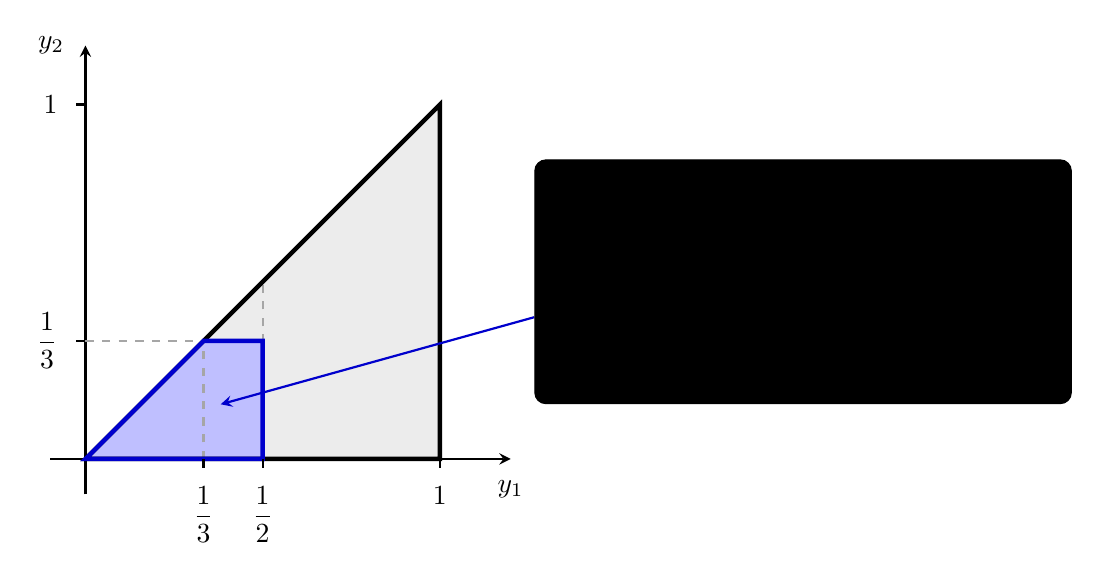
\begin{tikzpicture}[scale=1.5]
    % 1) Backgrounds / Shaded Regions
    \fill[gray!15] (0,0) -- (3,0) -- (3,3) -- cycle;
    \fill[blue!25] (0,0) -- (1.5,0) -- (1.5,1) -- (1,1) -- cycle;

    % 2) Grid Lines and Axes
    \draw[->, thick, >=stealth] (-0.3,0) -- (3.6,0) node[below=4pt, black] {$\displaystyle y_1$};
    \draw[->, thick, >=stealth] (0,-0.3) -- (0,3.5) node[left=4pt, black] {$\displaystyle y_2$};
    \draw[dashed, gray!70, thick] (1,0) -- (1,1);
    \draw[dashed, gray!70, thick] (0,1) -- (1.5,1);
    \draw[dashed, gray!70, thick] (1.5,0) -- (1.5,1.5);

    % 3) Primary Plots / Support Boundaries
    \draw[ultra thick, black] (0,0) -- (3,0) -- (3,3) -- cycle;
    \draw[ultra thick, blue!80!black] (0,0) -- (1.5,0) -- (1.5,1) -- (1,1) -- cycle;

    % 4) Node Labels, Tick Marks, and Callouts
    \draw[thick] (1,0) -- (1,-0.08) node[below=3pt, black] {$\displaystyle \frac{1}{3}$};
    \draw[thick] (1.5,0) -- (1.5,-0.08) node[below=3pt, black] {$\displaystyle \frac{1}{2}$};
    \draw[thick] (3,0) -- (3,-0.08) node[below=3pt, black] {$\displaystyle 1$};
    \draw[thick] (0,1) -- (-0.08,1) node[left=3pt, black] {$\displaystyle \frac{1}{3}$};
    \draw[thick] (0,3) -- (-0.08,3) node[left=3pt, black] {$\displaystyle 1$};

    \draw[->, >=stealth, shorten >=2pt, thick, blue!80!black] (3.8, 1.2) -- (1.1, 0.45);
    \node[draw, rounded corners, fill=white, align=left, inner sep=8pt, anchor=west, black] at (3.8, 1.5) {
        \textbf{Integration Domain (Exercise 5.5a)}\\[4pt]
        $\displaystyle \mathcal{S} = \{0 \le y_2 \le y_1 \le 1\}$ (Gray)\\
        $\displaystyle R_a = \mathcal{S} \cap \left\{y_1 \le \frac{1}{2},\ y_2 \le \frac{1}{3}\right\}$ (Blue)\\
        $\displaystyle \text{Horizontal slice: } y_2 \le y_1 \le \frac{1}{2}$
    };
\end{tikzpicture}
\end{center}

\textbf{Part (a): Evaluation of $F(1/2, 1/3)$.}
The effective domain of integration is $R_a = \mathcal{S} \cap ((-\infty, 1/2] \times (-\infty, 1/3]) = \{(y_1, y_2) \in \mathbb{R}^2 : 0 \le y_2 \le 1/3,\ y_2 \le y_1 \le 1/2\}$. Applying Tonelli's Theorem to integrate with respect to $y_1$ first (horizontally from $y_1 = y_2$ to $y_1 = 1/2$) and then with respect to $y_2$ from $0$ to $1/3$:
\begin{align*}
    F\!\left(\frac{1}{2}, \frac{1}{3}\right) &= \int_{0}^{1/3} \int_{y_2}^{1/2} 3y_1 \, dy_1 \, dy_2 \\
    &= \int_{0}^{1/3} \left[ \frac{3}{2} y_1^2 \right]_{y_1 = y_2}^{y_1 = 1/2} dy_2 \\
    &= \frac{3}{2} \int_{0}^{1/3} \left( \frac{1}{4} - y_2^2 \right) dy_2 \\
    &= \frac{3}{2} \left[ \frac{1}{4} y_2 - \frac{1}{3} y_2^3 \right]_{0}^{1/3} \\
    &= \frac{3}{2} \left( \frac{1}{12} - \frac{1}{81} \right) = \frac{1}{8} - \frac{1}{54} = \frac{27 - 4}{216} = \frac{23}{216}.
\end{align*}

\textbf{Part (b): Evaluation of $\mathbb{P}(Y_2 \le Y_1/2)$.}
Since $\frac{1}{2} y_1 \le y_1$ for all $y_1 \in [0, 1]$, the intersection of $\{y_2 \le y_1/2\}$ with the support $\mathcal{S}$ is the triangular wedge $R_b = \{(y_1, y_2) \in \mathbb{R}^2 : 0 \le y_1 \le 1,\ 0 \le y_2 \le y_1/2\}$. Integrating with respect to $y_2$ first:
\begin{align*}
    \mathbb{P}\!\left(Y_2 \le \frac{Y_1}{2}\right) &= \int_{0}^{1} \int_{0}^{y_1/2} 3y_1 \, dy_2 \, dy_1 \\
    &= \int_{0}^{1} 3y_1 \left[ y_2 \right]_{0}^{y_1/2} dy_1 \\
    &= \int_{0}^{1} \frac{3}{2} y_1^2 \, dy_1 = \left[ \frac{1}{2} y_1^3 \right]_{0}^{1} = \frac{1}{2}.
\end{align*}
\textbf{Final Answer:} \textbf{(a)} $F(1/2, 1/3) = \dfrac{23}{216}$; \quad \textbf{(b)} $\mathbb{P}(Y_2 \le Y_1/2) = \dfrac{1}{2}$. $\blacksquare$

\bigskip

\subsubsection*{Exercise 5.6}
\textbf{Original Problem:} Refer to Example 5.3. If a radioactive particle is randomly located in a square of unit length, a reasonable model for the joint density function for $Y_1$ and $Y_2$ is
\[
    f(y_1, y_2) = \begin{cases}
        1, & 0 \le y_1 \le 1,\ 0 \le y_2 \le 1, \\
        0, & \text{elsewhere.}
    \end{cases}
\]
\begin{enumerate}[label=\textbf{\alph*}]
    \item What is $P(Y_1 - Y_2 > .5)$?
    \item What is $P(Y_1 Y_2 < .5)$?
\end{enumerate}

\textbf{Rigorous Solution:}

\textbf{Part (a): Evaluation of $\mathbb{P}(Y_1 - Y_2 > 0.5)$.}
Within the unit square $\mathcal{S} = [0, 1]^2$, the inequality $y_1 - y_2 > \frac{1}{2}$ is equivalent to $y_2 < y_1 - \frac{1}{2}$. Since $y_2 \ge 0$, we must have $y_1 - \frac{1}{2} > 0 \implies y_1 > \frac{1}{2}$. Thus, the region of integration is $R_a = \{(y_1, y_2) : \frac{1}{2} < y_1 \le 1,\ 0 \le y_2 < y_1 - \frac{1}{2}\}$:
\begin{align*}
    \mathbb{P}(Y_1 - Y_2 > 0.5) &= \int_{1/2}^{1} \int_{0}^{y_1 - 1/2} 1 \, dy_2 \, dy_1 \\
    &= \int_{1/2}^{1} \left( y_1 - \frac{1}{2} \right) dy_1 \\
    &= \left[ \frac{1}{2} \left( y_1 - \frac{1}{2} \right)^2 \right]_{1/2}^{1} = \frac{1}{2} \left(\frac{1}{2}\right)^2 = \frac{1}{8} = 0.125.
\end{align*}

\textbf{Part (b): Evaluation of $\mathbb{P}(Y_1 Y_2 < 0.5)$.}
Within $\mathcal{S} = [0, 1]^2$, the hyperbolic boundary $y_1 y_2 = \frac{1}{2} \iff y_2 = \frac{1}{2y_1}$ intersects the top boundary $y_2 = 1$ at $y_1 = \frac{1}{2}$ and the right boundary $y_1 = 1$ at $y_2 = \frac{1}{2}$.
\begin{itemize}
    \item For $0 \le y_1 \le \frac{1}{2}$, since $y_2 \le 1$, we automatically have $y_1 y_2 \le \frac{1}{2} (1) = \frac{1}{2}$. Thus $y_2$ ranges from $0$ to $1$.
    \item For $\frac{1}{2} < y_1 \le 1$, the upper bound on $y_2$ is constrained by the hyperbola $y_2 = \frac{1}{2y_1}$.
\end{itemize}
Splitting the integral across these two disjoint sub-domains:
\begin{align*}
    \mathbb{P}(Y_1 Y_2 < 0.5) &= \int_{0}^{1/2} \int_{0}^{1} 1 \, dy_2 \, dy_1 + \int_{1/2}^{1} \int_{0}^{\frac{1}{2y_1}} 1 \, dy_2 \, dy_1 \\
    &= \int_{0}^{1/2} 1 \, dy_1 + \int_{1/2}^{1} \frac{1}{2y_1} \, dy_1 \\
    &= \frac{1}{2} + \frac{1}{2} \Bigl[ \ln(y_1) \Bigr]_{1/2}^{1} \\
    &= \frac{1}{2} + \frac{1}{2} \bigl( \ln(1) - \ln(1/2) \bigr) = \frac{1 + \ln 2}{2} \approx 0.84657.
\end{align*}
\textbf{Final Answer:} \textbf{(a)} $\mathbb{P}(Y_1 - Y_2 > 0.5) = \dfrac{1}{8} = 0.125$; \quad \textbf{(b)} $\mathbb{P}(Y_1 Y_2 < 0.5) = \dfrac{1 + \ln 2}{2} \approx 0.8466$. $\blacksquare$

\bigskip

\subsubsection*{Exercise 5.7}
\textbf{Original Problem:} Let $Y_1$ and $Y_2$ have joint density function
\[
    f(y_1, y_2) = \begin{cases}
        e^{-(y_1 + y_2)}, & y_1 > 0,\ y_2 > 0, \\
        0, & \text{elsewhere.}
    \end{cases}
\]
\begin{enumerate}[label=\textbf{\alph*}]
    \item What is $P(Y_1 < 1, Y_2 > 5)$?
    \item What is $P(Y_1 + Y_2 < 3)$?
\end{enumerate}

\textbf{Rigorous Solution:}

\textbf{Part (a): Evaluation of $\mathbb{P}(Y_1 < 1, Y_2 > 5)$.}
The region of integration intersected with the first quadrant $\mathcal{S} = (0, \infty)^2$ is the Cartesian product $(0, 1) \times (5, \infty)$. Since the integrand factors into $e^{-y_1} e^{-y_2}$ over a rectangular product domain, Fubini's Theorem yields:
\begin{align*}
    \mathbb{P}(Y_1 < 1, Y_2 > 5) &= \int_{0}^{1} \int_{5}^{\infty} e^{-(y_1 + y_2)} \, dy_2 \, dy_1 \\
    &= \left( \int_{0}^{1} e^{-y_1} \, dy_1 \right) \left( \int_{5}^{\infty} e^{-y_2} \, dy_2 \right) \\
    &= \Bigl[ -e^{-y_1} \Bigr]_{0}^{1} \cdot \left( \lim_{b \to \infty} \Bigl[ -e^{-y_2} \Bigr]_{5}^{b} \right) \\
    &= \left( 1 - e^{-1} \right) e^{-5} = e^{-5} - e^{-6} \approx 0.004259.
\end{align*}

\textbf{Part (b): Evaluation of $\mathbb{P}(Y_1 + Y_2 < 3)$.}
Intersecting $y_1 + y_2 < 3$ with $y_1 > 0, y_2 > 0$ gives the simplex $R_b = \{(y_1, y_2) : 0 < y_1 < 3,\ 0 < y_2 < 3 - y_1\}$:
\begin{align*}
    \mathbb{P}(Y_1 + Y_2 < 3) &= \int_{0}^{3} \int_{0}^{3 - y_1} e^{-y_1} e^{-y_2} \, dy_2 \, dy_1 \\
    &= \int_{0}^{3} e^{-y_1} \Bigl[ -e^{-y_2} \Bigr]_{0}^{3 - y_1} dy_1 \\
    &= \int_{0}^{3} e^{-y_1} \left( 1 - e^{-(3 - y_1)} \right) dy_1 \\
    &= \int_{0}^{3} \left( e^{-y_1} - e^{-3} \right) dy_1 \\
    &= \Bigl[ -e^{-y_1} - y_1 e^{-3} \Bigr]_{0}^{3} \\
    &= \left( -e^{-3} - 3e^{-3} \right) - (-1 - 0) = 1 - 4e^{-3} \approx 0.80085.
\end{align*}
\textbf{Final Answer:} \textbf{(a)} $\mathbb{P}(Y_1 < 1, Y_2 > 5) = e^{-5}(1 - e^{-1}) = e^{-5} - e^{-6}$; \quad \textbf{(b)} $\mathbb{P}(Y_1 + Y_2 < 3) = 1 - 4e^{-3}$. $\blacksquare$

\bigskip

\subsubsection*{Exercise 5.8}
\textbf{Original Problem:} Let $Y_1$ and $Y_2$ have the joint probability density function given by
\[
    f(y_1, y_2) = \begin{cases}
        k y_1 y_2, & 0 \le y_1 \le 1,\ 0 \le y_2 \le 1, \\
        0, & \text{elsewhere.}
    \end{cases}
\]
\begin{enumerate}[label=\textbf{\alph*}]
    \item Find the value of $k$ that makes this a probability density function.
    \item Find the joint distribution function for $Y_1$ and $Y_2$.
    \item Find $P(Y_1 \le 1/2, Y_2 \le 3/4)$.
\end{enumerate}

\textbf{Rigorous Solution:}

\textbf{Part (a): Determination of the Normalizing Constant $k$.}
By Theorem 5.2b, $f(y_1, y_2)$ is a valid PDF if and only if $k \ge 0$ and $\int_{-\infty}^\infty \int_{-\infty}^\infty f(y_1, y_2) \, dy_1 \, dy_2 = 1$:
\begin{align*}
    1 &= \int_{0}^{1} \int_{0}^{1} k y_1 y_2 \, dy_1 \, dy_2 \\
    &= k \left( \int_{0}^{1} y_1 \, dy_1 \right) \left( \int_{0}^{1} y_2 \, dy_2 \right) \\
    &= k \left( \frac{1}{2} \right) \left( \frac{1}{2} \right) = \frac{k}{4} \implies k = 4.
\end{align*}

\textbf{Part (b): Derivation of the Joint CDF $F(y_1, y_2)$ Across $\mathbb{R}^2$.}
By Definition 5.3, $F(y_1, y_2) = \int_{-\infty}^{y_1} \int_{-\infty}^{y_2} f(t_1, t_2) \, dt_2 \, dt_1$. Because the support is $[0, 1]^2$, we partition $\mathbb{R}^2$ into five regions:
\begin{itemize}
    \item If $y_1 < 0$ or $y_2 < 0$, the region $(-\infty, y_1] \times (-\infty, y_2]$ does not intersect $(0, 1]^2$, so $F(y_1, y_2) = 0$.
    \item If $0 \le y_1 \le 1$ and $0 \le y_2 \le 1$:
    \[
        F(y_1, y_2) = \int_{0}^{y_1} \int_{0}^{y_2} 4 t_1 t_2 \, dt_2 \, dt_1 = \left( \int_{0}^{y_1} 2t_1 \, dt_1 \right) \left( \int_{0}^{y_2} 2t_2 \, dt_2 \right) = y_1^2 y_2^2.
    \]
    \item If $0 \le y_1 \le 1$ and $y_2 > 1$, the upper limit for $t_2$ caps at $1$, yielding $F(y_1, y_2) = y_1^2 (1)^2 = y_1^2$.
    \item If $y_1 > 1$ and $0 \le y_2 \le 1$, the upper limit for $t_1$ caps at $1$, yielding $F(y_1, y_2) = (1)^2 y_2^2 = y_2^2$.
    \item If $y_1 > 1$ and $y_2 > 1$, the entire support is covered, yielding $F(y_1, y_2) = 1$.
\end{itemize}
Summarizing in piecewise form:
\[
    F(y_1, y_2) = \begin{cases}
        0, & \text{if } y_1 < 0 \text{ or } y_2 < 0, \\
        y_1^2 y_2^2, & \text{if } 0 \le y_1 \le 1 \text{ and } 0 \le y_2 \le 1, \\
        y_1^2, & \text{if } 0 \le y_1 \le 1 \text{ and } y_2 > 1, \\
        y_2^2, & \text{if } y_1 > 1 \text{ and } 0 \le y_2 \le 1, \\
        1, & \text{if } y_1 > 1 \text{ and } y_2 > 1.
    \end{cases}
\]

\textbf{Part (c): Evaluation of $\mathbb{P}(Y_1 \le 1/2, Y_2 \le 3/4)$.}
Using the joint CDF derived in Part (b) for $(1/2, 3/4) \in [0, 1]^2$:
\[
    \mathbb{P}\!\left(Y_1 \le \frac{1}{2}, Y_2 \le \frac{3}{4}\right) = F\!\left(\frac{1}{2}, \frac{3}{4}\right) = \left(\frac{1}{2}\right)^2 \left(\frac{3}{4}\right)^2 = \frac{1}{4} \cdot \frac{9}{16} = \frac{9}{64}.
\]
\textbf{Final Answer:} \textbf{(a)} $k = 4$; \quad \textbf{(b)} $F(y_1, y_2) = y_1^2 y_2^2$ on $[0,1]^2$ (with boundary extensions above); \quad \textbf{(c)} $\dfrac{9}{64}$. $\blacksquare$

\bigskip

\subsubsection*{Exercise 5.9}
\textbf{Original Problem:} Let $Y_1$ and $Y_2$ have the joint probability density function given by
\[
    f(y_1, y_2) = \begin{cases}
        k(1 - y_2), & 0 \le y_1 \le y_2 \le 1, \\
        0, & \text{elsewhere.}
    \end{cases}
\]
\begin{enumerate}[label=\textbf{\alph*}]
    \item Find the value of $k$ that makes this a probability density function.
    \item Find $P(Y_1 \le 3/4, Y_2 \ge 1/2)$.
\end{enumerate}

\textbf{Rigorous Solution:}

\textbf{Part (a): Determination of $k$.}
Imposing the normalization condition $\iint_{\mathcal{S}} f(y_1, y_2) \, dy_1 \, dy_2 = 1$ over $\mathcal{S} = \{0 \le y_1 \le y_2 \le 1\}$:
\begin{align*}
    1 &= \int_{0}^{1} \int_{0}^{y_2} k(1 - y_2) \, dy_1 \, dy_2 \\
    &= k \int_{0}^{1} (1 - y_2) \Bigl[ y_1 \Bigr]_{0}^{y_2} dy_2 \\
    &= k \int_{0}^{1} \left( y_2 - y_2^2 \right) dy_2 \\
    &= k \left[ \frac{1}{2} y_2^2 - \frac{1}{3} y_2^3 \right]_{0}^{1} = k \left( \frac{1}{2} - \frac{1}{3} \right) = \frac{k}{6} \implies k = 6.
\end{align*}

\textbf{Part (b): Evaluation of $\mathbb{P}(Y_1 \le 3/4, Y_2 \ge 1/2)$.}
Within the support $0 \le y_1 \le y_2 \le 1$, we require $y_2 \ge 1/2$ and $y_1 \le \min(y_2, 3/4)$. Thus, we partition the outer integral over $y_2 \in [1/2, 1]$ into two sub-intervals:
\begin{itemize}
    \item For $\frac{1}{2} \le y_2 \le \frac{3}{4}$, $\min(y_2, 3/4) = y_2$, so $0 \le y_1 \le y_2$.
    \item For $\frac{3}{4} < y_2 \le 1$, $\min(y_2, 3/4) = \frac{3}{4}$, so $0 \le y_1 \le \frac{3}{4}$.
\end{itemize}
Evaluating the sum of these two iterated integrals with $k = 6$:
\begin{align*}
    \mathbb{P}\!\left(Y_1 \le \frac{3}{4}, Y_2 \ge \frac{1}{2}\right) 
    &= \int_{1/2}^{3/4} \int_{0}^{y_2} 6(1 - y_2) \, dy_1 \, dy_2 + \int_{3/4}^{1} \int_{0}^{3/4} 6(1 - y_2) \, dy_1 \, dy_2 \\
    &= \int_{1/2}^{3/4} \left( 6y_2 - 6y_2^2 \right) dy_2 + \frac{3}{4} \int_{3/4}^{1} 6(1 - y_2) \, dy_2 \\
    &= \Bigl[ 3y_2^2 - 2y_2^3 \Bigr]_{1/2}^{3/4} + \frac{9}{2} \left[ -\frac{1}{2}(1 - y_2)^2 \right]_{3/4}^{1} \\
    &= \left[ \left( 3 \cdot \frac{9}{16} - 2 \cdot \frac{27}{64} \right) - \left( 3 \cdot \frac{1}{4} - 2 \cdot \frac{1}{8} \right) \right] + \frac{9}{4} \left( \frac{1}{16} \right) \\
    &= \left( \frac{27}{32} - \frac{1}{2} \right) + \frac{9}{64} = \frac{11}{32} + \frac{9}{64} = \frac{22 + 9}{64} = \frac{31}{64}.
\end{align*}
\textbf{Final Answer:} \textbf{(a)} $k = 6$; \quad \textbf{(b)} $\mathbb{P}(Y_1 \le 3/4, Y_2 \ge 1/2) = \dfrac{31}{64}$. $\blacksquare$

\bigskip

\subsubsection*{Exercise 5.10}
\textbf{Original Problem:} An environmental engineer measures the amount (by weight) of particulate pollution in air samples of a certain volume collected over two smokestacks at a coal-operated power plant. One of the stacks is equipped with a cleaning device. Let $Y_1$ denote the amount of pollutant per sample collected above the stack that has no cleaning device and let $Y_2$ denote the amount of pollutant per sample collected above the stack that is equipped with the cleaning device. Suppose that the relative frequency behavior of $Y_1$ and $Y_2$ can be modeled by
\[
    f(y_1, y_2) = \begin{cases}
        k, & 0 \le y_1 \le 2,\ 0 \le y_2 \le 1,\ 2y_2 \le y_1, \\
        0, & \text{elsewhere.}
    \end{cases}
\]
That is, $Y_1$ and $Y_2$ are uniformly distributed over the region inside the triangle bounded by $y_1 = 2$, $y_2 = 0$, and $2y_2 = y_1$.
\begin{enumerate}[label=\textbf{\alph*}]
    \item Find the value of $k$ that makes this function a probability density function.
    \item Find $P(Y_1 \ge 3Y_2)$. That is, find the probability that the cleaning device reduces the amount of pollutant by one-third or more.
\end{enumerate}

\textbf{Rigorous Solution:}

\textbf{Part (a): Determination of $k$.}
The support $\mathcal{S} = \{(y_1, y_2) : 0 \le y_1 \le 2,\ 0 \le y_2 \le y_1/2\}$ is a right triangle with base $2$ and height $1$. Integrating $f(y_1, y_2) = k$ over $\mathcal{S}$:
\[
    1 = \int_{0}^{2} \int_{0}^{y_1/2} k \, dy_2 \, dy_1 = k \int_{0}^{2} \frac{y_1}{2} \, dy_1 = k \left[ \frac{y_1^2}{4} \right]_{0}^{2} = k(1) \implies k = 1.
\]

\textbf{Part (b): Evaluation of $\mathbb{P}(Y_1 \ge 3Y_2)$.}
The inequality $Y_1 \ge 3Y_2$ is equivalent to $Y_2 \le \frac{1}{3} Y_1$. Because $\frac{1}{3} y_1 \le \frac{1}{2} y_1$ for all $y_1 \ge 0$, the wedge $0 \le y_2 \le \frac{1}{3} y_1$ for $0 \le y_1 \le 2$ lies completely inside the support $\mathcal{S}$. Integrating $f(y_1, y_2) = 1$ over this region:
\begin{align*}
    \mathbb{P}(Y_1 \ge 3Y_2) &= \int_{0}^{2} \int_{0}^{y_1/3} 1 \, dy_2 \, dy_1 \\
    &= \int_{0}^{2} \frac{y_1}{3} \, dy_1 = \left[ \frac{y_1^2}{6} \right]_{0}^{2} = \frac{4}{6} = \frac{2}{3}.
\end{align*}
\textbf{Final Answer:} \textbf{(a)} $k = 1$; \quad \textbf{(b)} $\mathbb{P}(Y_1 \ge 3Y_2) = \dfrac{2}{3}$. $\blacksquare$

\bigskip

\subsubsection*{Exercise 5.11}
\textbf{Original Problem:} Suppose that $Y_1$ and $Y_2$ are uniformly distributed over the triangle shaded in the accompanying diagram (with vertices at $(-1, 0)$, $(1, 0)$, and $(0, 1)$).
\begin{enumerate}[label=\textbf{\alph*}]
    \item Find $P(Y_1 \le 3/4, Y_2 \le 3/4)$.
    \item Find $P(Y_1 - Y_2 \ge 0)$.
\end{enumerate}

\textbf{Rigorous Solution:}

\textbf{Derivation of the Joint Density Function:}
The support $\mathcal{S}$ is the triangle with vertices $(-1, 0)$, $(1, 0)$, and $(0, 1)$, bounded below by $y_2 = 0$, on the left by $y_2 = y_1 + 1 \iff y_1 = y_2 - 1$, and on the right by $y_2 = 1 - y_1 \iff y_1 = 1 - y_2$. The area of $\mathcal{S}$ is $\text{Area}(\mathcal{S}) = \frac{1}{2} \times \text{base} \times \text{height} = \frac{1}{2}(2)(1) = 1$. Since $(Y_1, Y_2)$ is uniformly distributed over $\mathcal{S}$, its constant density is $f(y_1, y_2) = \frac{1}{\text{Area}(\mathcal{S})} = 1$ on $\mathcal{S}$, and $0$ elsewhere.

\begin{center}
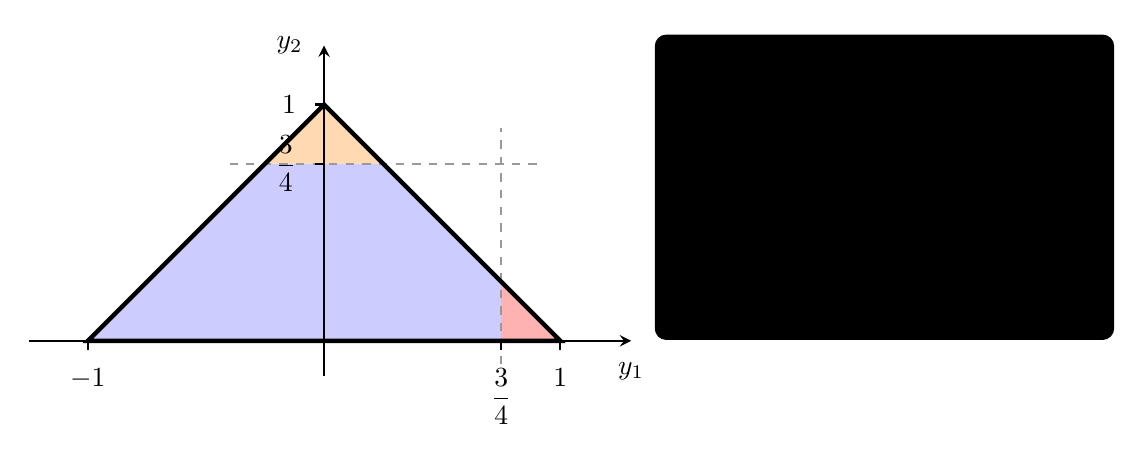
\begin{tikzpicture}[scale=1.5]
    % 1) Backgrounds / Shaded Regions
    \fill[blue!20] (-2,0) -- (1.5,0) -- (1.5,0.5) -- (0.5,1.5) -- (-0.5,1.5) -- cycle;
    \fill[red!30] (1.5,0) -- (2,0) -- (1.5,0.5) -- cycle;
    \fill[orange!30] (-0.5,1.5) -- (0.5,1.5) -- (0,2) -- cycle;

    % 2) Grid Lines and Axes
    \draw[->, thick, >=stealth] (-2.5,0) -- (2.6,0) node[below=4pt, black] {$\displaystyle y_1$};
    \draw[->, thick, >=stealth] (0,-0.3) -- (0,2.5) node[left=4pt, black] {$\displaystyle y_2$};
    \draw[dashed, thick, gray!80] (-0.8,1.5) -- (1.8,1.5);
    \draw[dashed, thick, gray!80] (1.5,-0.2) -- (1.5,1.8);

    % 3) Primary Plots
    \draw[ultra thick, black] (-2,0) -- (2,0) -- (0,2) -- cycle;

    % 4) Node Labels, Tick Marks, and Callouts
    \draw[thick] (-2,0) -- (-2,-0.08) node[below=3pt, black] {$\displaystyle -1$};
    \draw[thick] (1.5,0) -- (1.5,-0.08) node[below=3pt, black] {$\displaystyle \frac{3}{4}$};
    \draw[thick] (2,0) -- (2,-0.08) node[below=3pt, black] {$\displaystyle 1$};
    \draw[thick] (0,1.5) -- (-0.08,1.5) node[left=3pt, black] {$\displaystyle \frac{3}{4}$};
    \draw[thick] (0,2) -- (-0.08,2) node[left=3pt, black] {$\displaystyle 1$};

    \node[draw, rounded corners, fill=white, align=left, inner sep=8pt, anchor=west, black] at (2.8, 1.3) {
        \textbf{Exercise 5.11a Partition}\\[4pt]
        $\displaystyle \text{Blue: } \left\{Y_1 \le \frac{3}{4},\ Y_2 \le \frac{3}{4}\right\}$\\[4pt]
        $\displaystyle \text{Orange: } \left\{Y_2 > \frac{3}{4}\right\} \left(\text{Area} = \frac{1}{16}\right)$\\[4pt]
        $\displaystyle \text{Red: } \left\{Y_1 > \frac{3}{4}\right\} \left(\text{Area} = \frac{1}{32}\right)$
    };
\end{tikzpicture}
\end{center}

\textbf{Part (a): Evaluation of $\mathbb{P}(Y_1 \le 3/4, Y_2 \le 3/4)$.}
We provide both the direct integration proof and the set-theoretic complement proof:
\begin{itemize}
    \item \textbf{Method 1 (Direct Iterated Integration):} For $0 \le y_2 \le \frac{1}{4}$, the right boundary of the triangle is $1 - y_2 \ge \frac{3}{4}$, so $y_1$ is capped at $\frac{3}{4}$. For $\frac{1}{4} \le y_2 \le \frac{3}{4}$, $1 - y_2 \le \frac{3}{4}$, so $y_1$ runs up to $1 - y_2$:
    \begin{align*}
        \mathbb{P}\!\left(Y_1 \le \frac{3}{4}, Y_2 \le \frac{3}{4}\right) 
        &= \int_{0}^{1/4} \int_{y_2 - 1}^{3/4} 1 \, dy_1 \, dy_2 + \int_{1/4}^{3/4} \int_{y_2 - 1}^{1 - y_2} 1 \, dy_1 \, dy_2 \\
        &= \int_{0}^{1/4} \left( \frac{7}{4} - y_2 \right) dy_2 + \int_{1/4}^{3/4} (2 - 2y_2) \, dy_2 \\
        &= \left[ \frac{7}{4} y_2 - \frac{1}{2} y_2^2 \right]_{0}^{1/4} + \left[ 2y_2 - y_2^2 \right]_{1/4}^{3/4} \\
        &= \left( \frac{7}{16} - \frac{1}{32} \right) + \left[ \left( \frac{6}{4} - \frac{9}{16} \right) - \left( \frac{2}{4} - \frac{1}{16} \right) \right] = \frac{13}{32} + \frac{8}{16} = \frac{29}{32}.
    \end{align*}
    \item \textbf{Method 2 (De Morgan's Law and Complement Geometry):} Within $\mathcal{S}$, the complement of $\{Y_1 \le 3/4, Y_2 \le 3/4\}$ is $\{Y_1 > 3/4\} \cup \{Y_2 > 3/4\}$. Because $y_1 + y_2 \le 1$ on $\mathcal{S}$, these two events are mutually exclusive. The top triangle $\{Y_2 > 3/4\}$ has base $2(1 - 3/4) = 1/2$ and height $1/4$, so its area is $\frac{1}{2}(1/2)(1/4) = \frac{1}{16}$. The right corner triangle $\{Y_1 > 3/4\}$ has base $1/4$ and height $1/4$, so its area is $\frac{1}{2}(1/4)(1/4) = \frac{1}{32}$. Subtracting from $1$ gives $1 - \frac{1}{16} - \frac{1}{32} = \frac{29}{32}$.
\end{itemize}

\textbf{Part (b): Evaluation of $\mathbb{P}(Y_1 - Y_2 \ge 0)$.}
The inequality $Y_1 \ge Y_2$ inside $\mathcal{S}$ requires $y_2 \le y_1 \le 1 - y_2$. The lines $y_1 = y_2$ and $y_1 = 1 - y_2$ intersect at $(1/2, 1/2)$:
\begin{align*}
    \mathbb{P}(Y_1 - Y_2 \ge 0) &= \int_{0}^{1/2} \int_{y_2}^{1 - y_2} 1 \, dy_1 \, dy_2 \\
    &= \int_{0}^{1/2} (1 - 2y_2) \, dy_2 = \Bigl[ y_2 - y_2^2 \Bigr]_{0}^{1/2} = \frac{1}{2} - \frac{1}{4} = \frac{1}{4}.
\end{align*}
\textbf{Final Answer:} \textbf{(a)} $\mathbb{P}(Y_1 \le 3/4, Y_2 \le 3/4) = \dfrac{29}{32}$; \quad \textbf{(b)} $\mathbb{P}(Y_1 - Y_2 \ge 0) = \dfrac{1}{4}$. $\blacksquare$

\bigskip

\subsubsection*{Exercise 5.12}
\textbf{Original Problem:} Let $Y_1$ and $Y_2$ denote the proportions of two different types of components in a sample from a mixture of chemicals used as an insecticide. Suppose that $Y_1$ and $Y_2$ have the joint density function given by
\[
    f(y_1, y_2) = \begin{cases}
        2, & 0 \le y_1 \le 1,\ 0 \le y_2 \le 1,\ 0 \le y_1 + y_2 \le 1, \\
        0, & \text{elsewhere.}
    \end{cases}
\]
(Notice that $Y_1 + Y_2 \le 1$ because the random variables denote proportions within the same sample.) Find
\begin{enumerate}[label=\textbf{\alph*}]
    \item $P(Y_1 \le 3/4, Y_2 \le 3/4)$.
    \item $P(Y_1 \le 1/2, Y_2 \le 1/2)$.
\end{enumerate}

\textbf{Rigorous Solution:}

\textbf{Part (a): Evaluation of $\mathbb{P}(Y_1 \le 3/4, Y_2 \le 3/4)$.}
On the unit simplex $\mathcal{S} = \{(y_1, y_2) : y_1 \ge 0,\ y_2 \ge 0,\ y_1 + y_2 \le 1\}$, for $0 \le y_1 \le \frac{1}{4}$, the upper boundary $1 - y_1 \ge \frac{3}{4}$, so $y_2$ is capped at $\frac{3}{4}$. For $\frac{1}{4} \le y_1 \le \frac{3}{4}$, $y_2$ runs up to $1 - y_1$:
\begin{align*}
    \mathbb{P}\!\left(Y_1 \le \frac{3}{4}, Y_2 \le \frac{3}{4}\right) 
    &= \int_{0}^{1/4} \int_{0}^{3/4} 2 \, dy_2 \, dy_1 + \int_{1/4}^{3/4} \int_{0}^{1 - y_1} 2 \, dy_2 \, dy_1 \\
    &= 2 \left(\frac{1}{4}\right)\left(\frac{3}{4}\right) + \int_{1/4}^{3/4} 2(1 - y_1) \, dy_1 \\
    &= \frac{3}{8} + \Bigl[ -(1 - y_1)^2 \Bigr]_{1/4}^{3/4} \\
    &= \frac{3}{8} + \left( -\frac{1}{16} + \frac{9}{16} \right) = \frac{3}{8} + \frac{1}{2} = \frac{7}{8}.
\end{align*}

\textbf{Part (b): Evaluation of $\mathbb{P}(Y_1 \le 1/2, Y_2 \le 1/2)$.}
Observe that for every $(y_1, y_2) \in [0, 1/2] \times [0, 1/2]$, we have $0 \le y_1 + y_2 \le \frac{1}{2} + \frac{1}{2} = 1$. Therefore, the square $[0, 1/2] \times [0, 1/2]$ is a subset of the support $\mathcal{S}$:
\begin{align*}
    \mathbb{P}\!\left(Y_1 \le \frac{1}{2}, Y_2 \le \frac{1}{2}\right) 
    &= \int_{0}^{1/2} \int_{0}^{1/2} 2 \, dy_2 \, dy_1 \\
    &= 2 \left(\frac{1}{2}\right) \left(\frac{1}{2}\right) = \frac{1}{2}.
\end{align*}
\textbf{Final Answer:} \textbf{(a)} $\mathbb{P}(Y_1 \le 3/4, Y_2 \le 3/4) = \dfrac{7}{8}$; \quad \textbf{(b)} $\mathbb{P}(Y_1 \le 1/2, Y_2 \le 1/2) = \dfrac{1}{2}$. $\blacksquare$

\bigskip

\subsubsection*{Exercise 5.13}
\textbf{Original Problem:} The joint density function of $Y_1$ and $Y_2$ is given by
\[
    f(y_1, y_2) = \begin{cases}
        30 y_1 y_2^2, & y_1 - 1 \le y_2 \le 1 - y_1,\ 0 \le y_1 \le 1, \\
        0, & \text{elsewhere.}
    \end{cases}
\]
\begin{enumerate}[label=\textbf{\alph*}]
    \item Find $F(1/2, 1/2)$.
    \item Find $F(1/2, 2)$.
    \item Find $P(Y_1 > Y_2)$.
\end{enumerate}

\textbf{Rigorous Solution:}

\textbf{Part (a): Evaluation of $F(1/2, 1/2) = \mathbb{P}(Y_1 \le 1/2, Y_2 \le 1/2)$.}
For $0 \le y_1 \le \frac{1}{2}$, the upper support boundary satisfies $1 - y_1 \ge \frac{1}{2}$. Hence, intersecting the support with $y_2 \le \frac{1}{2}$ restricts $y_2$ to the interval $[y_1 - 1, 1/2]$:
\begin{align*}
    F\!\left(\frac{1}{2}, \frac{1}{2}\right) &= \int_{0}^{1/2} \int_{y_1 - 1}^{1/2} 30 y_1 y_2^2 \, dy_2 \, dy_1 \\
    &= \int_{0}^{1/2} 10 y_1 \Bigl[ y_2^3 \Bigr]_{y_1 - 1}^{1/2} dy_1 \\
    &= 10 \int_{0}^{1/2} y_1 \left( \frac{1}{8} - (y_1 - 1)^3 \right) dy_1 \\
    &= \frac{5}{4} \int_{0}^{1/2} y_1 \, dy_1 + 10 \int_{0}^{1/2} y_1 (1 - y_1)^3 \, dy_1.
\end{align*}
For the first integral, $\frac{5}{4} \left[\frac{1}{2}y_1^2\right]_0^{1/2} = \frac{5}{32}$. For the second integral, apply the substitution $u = 1 - y_1$ ($du = -dy_1$, $y_1 = 1 - u$), mapping $y_1 \in [0, 1/2]$ to $u \in [1/2, 1]$:
\begin{align*}
    10 \int_{1/2}^{1} (1 - u) u^3 \, du &= 10 \left[ \frac{u^4}{4} - \frac{u^5}{5} \right]_{1/2}^{1} \\
    &= 10 \left[ \left( \frac{1}{4} - \frac{1}{5} \right) - \left( \frac{1}{64} - \frac{1}{160} \right) \right] \\
    &= 10 \left( \frac{1}{20} - \frac{3}{320} \right) = 10 \left( \frac{13}{320} \right) = \frac{13}{32}.
\end{align*}
Adding the two components gives:
\[
    F\!\left(\frac{1}{2}, \frac{1}{2}\right) = \frac{5}{32} + \frac{13}{32} = \frac{18}{32} = \frac{9}{16}.
\]

\textbf{Part (b): Evaluation of $F(1/2, 2) = \mathbb{P}(Y_1 \le 1/2, Y_2 \le 2)$.}
Since the support $\mathcal{S}$ satisfies $y_2 \le 1 - y_1 \le 1 < 2$ for all $y_1 \in [0, 1]$, the condition $Y_2 \le 2$ places no additional restriction on $y_2$:
\begin{align*}
    F\!\left(\frac{1}{2}, 2\right) &= \int_{0}^{1/2} \int_{y_1 - 1}^{1 - y_1} 30 y_1 y_2^2 \, dy_2 \, dy_1 \\
    &= \int_{0}^{1/2} 10 y_1 \Bigl[ (1 - y_1)^3 - (y_1 - 1)^3 \Bigr] dy_1 \\
    &= 20 \int_{0}^{1/2} y_1 (1 - y_1)^3 \, dy_1 = 2 \left( \frac{13}{32} \right) = \frac{13}{16}.
\end{align*}

\textbf{Part (c): Evaluation of $\mathbb{P}(Y_1 > Y_2)$.}
Rather than splitting the region $\{y_2 < y_1\} \cap \mathcal{S}$ into two sub-integrals, we use the complement event $\{Y_2 \ge Y_1\} \cap \mathcal{S}$, which is a single triangle bounded by $0 \le y_1 \le \frac{1}{2}$ and $y_1 \le y_2 \le 1 - y_1$:
\begin{align*}
    \mathbb{P}(Y_2 \ge Y_1) &= \int_{0}^{1/2} \int_{y_1}^{1 - y_1} 30 y_1 y_2^2 \, dy_2 \, dy_1 \\
    &= 10 \int_{0}^{1/2} y_1 \left( (1 - y_1)^3 - y_1^3 \right) dy_1 \\
    &= 10 \int_{0}^{1/2} y_1 (1 - y_1)^3 \, dy_1 - 10 \int_{0}^{1/2} y_1^4 \, dy_1 \\
    &= \frac{13}{32} - \Bigl[ 2 y_1^5 \Bigr]_{0}^{1/2} = \frac{13}{32} - \frac{2}{32} = \frac{11}{32}.
\end{align*}
By the complement rule of probability measures,
\[
    \mathbb{P}(Y_1 > Y_2) = 1 - \mathbb{P}(Y_2 \ge Y_1) = 1 - \frac{11}{32} = \frac{21}{32}.
\]
\textbf{Final Answer:} \textbf{(a)} $F(1/2, 1/2) = \dfrac{9}{16}$; \quad \textbf{(b)} $F(1/2, 2) = \dfrac{13}{16}$; \quad \textbf{(c)} $\mathbb{P}(Y_1 > Y_2) = \dfrac{21}{32}$. $\blacksquare$

\bigskip

\subsubsection*{Exercise 5.14}
\textbf{Original Problem:} Suppose that the random variables $Y_1$ and $Y_2$ have joint probability density function $f(y_1, y_2)$ given by
\[
    f(y_1, y_2) = \begin{cases}
        6 y_1^2 y_2, & 0 \le y_1 \le y_2,\ y_1 + y_2 \le 2, \\
        0, & \text{elsewhere.}
    \end{cases}
\]
\begin{enumerate}[label=\textbf{\alph*}]
    \item Verify that this is a valid joint density function.
    \item What is the probability that $Y_1 + Y_2$ is less than $1$?
\end{enumerate}

\textbf{Rigorous Solution:}

\begin{center}
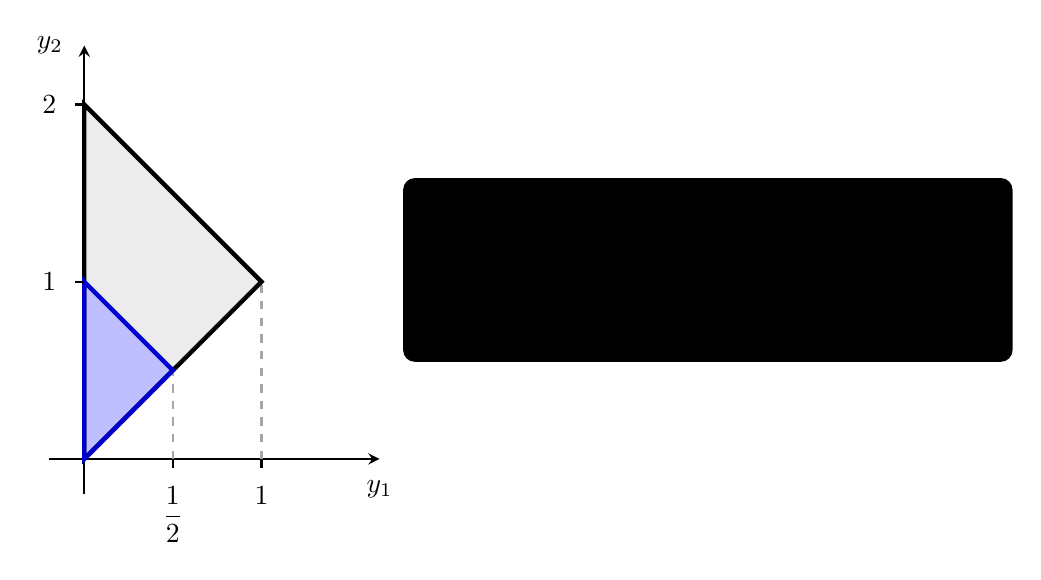
\begin{tikzpicture}[scale=1.5]
    % 1) Backgrounds / Shaded Regions
    \fill[gray!15] (0,0) -- (1.5,1.5) -- (0,3) -- cycle;
    \fill[blue!25] (0,0) -- (0.75,0.75) -- (0,1.5) -- cycle;

    % 2) Grid Lines and Axes
    \draw[->, thick, >=stealth] (-0.3,0) -- (2.5,0) node[below=4pt, black] {$\displaystyle y_1$};
    \draw[->, thick, >=stealth] (0,-0.3) -- (0,3.5) node[left=4pt, black] {$\displaystyle y_2$};
    \draw[dashed, gray!70, thick] (0.75,0) -- (0.75,0.75);
    \draw[dashed, gray!70, thick] (1.5,0) -- (1.5,1.5);

    % 3) Primary Plots
    \draw[ultra thick, black] (0,0) -- (1.5,1.5) -- (0,3) -- cycle;
    \draw[ultra thick, blue!80!black] (0,0) -- (0.75,0.75) -- (0,1.5) -- cycle;

    % 4) Node Labels, Tick Marks, and Callouts
    \draw[thick] (0.75,0) -- (0.75,-0.08) node[below=3pt, black] {$\displaystyle \frac{1}{2}$};
    \draw[thick] (1.5,0) -- (1.5,-0.08) node[below=3pt, black] {$\displaystyle 1$};
    \draw[thick] (0,1.5) -- (-0.08,1.5) node[left=3pt, black] {$\displaystyle 1$};
    \draw[thick] (0,3) -- (-0.08,3) node[left=3pt, black] {$\displaystyle 2$};

    \node[draw, rounded corners, fill=white, align=left, inner sep=8pt, anchor=west, black] at (2.7, 1.6) {
        \textbf{Exercise 5.14 Integration Domains}\\[4pt]
        $\displaystyle \text{Support } \mathcal{S}: 0 \le y_1 \le 1,\ y_1 \le y_2 \le 2 - y_1$\\[4pt]
        $\displaystyle \text{Sub-domain } R_b: 0 \le y_1 \le \frac{1}{2},\ y_1 \le y_2 \le 1 - y_1$
    };
\end{tikzpicture}
\end{center}

\textbf{Part (a): Verification of Theorem 5.2b.}
\begin{enumerate}[label=\arabic*.]
    \item \textbf{Non-Negativity:} On the support $\mathcal{S} = \{(y_1, y_2) : 0 \le y_1 \le y_2,\ y_1 + y_2 \le 2\}$, we have $y_1^2 \ge 0$ and $y_2 \ge 0$, so $f(y_1, y_2) = 6y_1^2 y_2 \ge 0$ everywhere.
    \item \textbf{Normalization:} The boundary lines $y_2 = y_1$ and $y_2 = 2 - y_1$ intersect at $y_1 = 2 - y_1 \implies (y_1, y_2) = (1, 1)$. Thus $\mathcal{S}$ is parameterized by $0 \le y_1 \le 1$ and $y_1 \le y_2 \le 2 - y_1$. Integrating $f$ over $\mathcal{S}$:
    \begin{align*}
        \iint_{\mathcal{S}} 6 y_1^2 y_2 \, dy_2 \, dy_1 
        &= \int_{0}^{1} \int_{y_1}^{2 - y_1} 6 y_1^2 y_2 \, dy_2 \, dy_1 \\
        &= \int_{0}^{1} 3 y_1^2 \Bigl[ y_2^2 \Bigr]_{y_1}^{2 - y_1} dy_1 \\
        &= \int_{0}^{1} 3 y_1^2 \left( (2 - y_1)^2 - y_1^2 \right) dy_1 \\
        &= \int_{0}^{1} 3 y_1^2 (4 - 4y_1) \, dy_1 \\
        &= \int_{0}^{1} \left( 12 y_1^2 - 12 y_1^3 \right) dy_1 = \Bigl[ 4 y_1^3 - 3 y_1^4 \Bigr]_{0}^{1} = 4 - 3 = 1.
    \end{align*}
\end{enumerate}
Hence, $f(y_1, y_2)$ is a valid joint probability density function.

\textbf{Part (b): Evaluation of $\mathbb{P}(Y_1 + Y_2 < 1)$.}
Intersecting $y_1 + y_2 < 1$ with $0 \le y_1 \le y_2$ yields the smaller triangle bounded by $y_2 = y_1$ and $y_2 = 1 - y_1$, which intersect at $(1/2, 1/2)$:
\begin{align*}
    \mathbb{P}(Y_1 + Y_2 < 1) &= \int_{0}^{1/2} \int_{y_1}^{1 - y_1} 6 y_1^2 y_2 \, dy_2 \, dy_1 \\
    &= \int_{0}^{1/2} 3 y_1^2 \left( (1 - y_1)^2 - y_1^2 \right) dy_1 \\
    &= \int_{0}^{1/2} 3 y_1^2 (1 - 2y_1) \, dy_1 \\
    &= \int_{0}^{1/2} \left( 3 y_1^2 - 6 y_1^3 \right) dy_1 \\
    &= \left[ y_1^3 - \frac{3}{2} y_1^4 \right]_{0}^{1/2} = \frac{1}{8} - \frac{3}{2}\left(\frac{1}{16}\right) = \frac{4 - 3}{32} = \frac{1}{32}.
\end{align*}
\textbf{Final Answer:} \textbf{(a)} Verified above; \quad \textbf{(b)} $\mathbb{P}(Y_1 + Y_2 < 1) = \dfrac{1}{32}$. $\blacksquare$

\bigskip

\subsubsection*{Exercise 5.15}
\textbf{Original Problem:} The management at a fast-food outlet is interested in the joint behavior of the random variables $Y_1$, defined as the total time between a customer's arrival at the store and departure from the service window, and $Y_2$, the time a customer waits in line before reaching the service window. Because $Y_1$ includes the time a customer waits in line, we must have $Y_1 \ge Y_2$. The relative frequency distribution of observed values of $Y_1$ and $Y_2$ can be modeled by the probability density function
\[
    f(y_1, y_2) = \begin{cases}
        e^{-y_1}, & 0 \le y_2 \le y_1 < \infty, \\
        0, & \text{elsewhere}
    \end{cases}
\]
with time measured in minutes. Find
\begin{enumerate}[label=\textbf{\alph*}]
    \item $P(Y_1 < 2, Y_2 > 1)$.
    \item $P(Y_1 \ge 2Y_2)$.
    \item $P(Y_1 - Y_2 \ge 1)$. (Notice that $Y_1 - Y_2$ denotes the time spent at the service window.)
\end{enumerate}

\textbf{Rigorous Solution:}

\textbf{Part (a): Evaluation of $\mathbb{P}(Y_1 < 2, Y_2 > 1)$.}
Intersecting $\{y_1 < 2,\ y_2 > 1\}$ with the support $\{0 \le y_2 \le y_1 < \infty\}$ yields the triangular domain $1 < y_2 \le y_1 < 2$. Integrating with respect to $y_2$ first:
\begin{align*}
    \mathbb{P}(Y_1 < 2, Y_2 > 1) &= \int_{1}^{2} \int_{1}^{y_1} e^{-y_1} \, dy_2 \, dy_1 \\
    &= \int_{1}^{2} (y_1 - 1) e^{-y_1} \, dy_1.
\end{align*}
Applying integration by parts with $u = y_1 - 1$ ($du = dy_1$) and $dv = e^{-y_1} dy_1$ ($v = -e^{-y_1}$):
\begin{align*}
    \int_{1}^{2} (y_1 - 1) e^{-y_1} \, dy_1 &= \Bigl[ -(y_1 - 1) e^{-y_1} \Bigr]_{1}^{2} + \int_{1}^{2} e^{-y_1} \, dy_1 \\
    &= \Bigl[ -y_1 e^{-y_1} \Bigr]_{1}^{2} = e^{-1} - 2e^{-2} \approx 0.09721.
\end{align*}

\textbf{Part (b): Evaluation of $\mathbb{P}(Y_1 \ge 2Y_2)$.}
The inequality $Y_1 \ge 2Y_2$ is equivalent to $0 \le y_2 \le \frac{1}{2} y_1$ for $0 \le y_1 < \infty$:
\begin{align*}
    \mathbb{P}(Y_1 \ge 2Y_2) &= \int_{0}^{\infty} \int_{0}^{y_1/2} e^{-y_1} \, dy_2 \, dy_1 \\
    &= \frac{1}{2} \int_{0}^{\infty} y_1 e^{-y_1} \, dy_1 = \frac{1}{2} \Gamma(2) = \frac{1}{2} (1!) = \frac{1}{2}.
\end{align*}

\textbf{Part (c): Evaluation of $\mathbb{P}(Y_1 - Y_2 \ge 1)$.}
The inequality $y_1 - y_2 \ge 1 \iff y_2 \le y_1 - 1$ together with $y_2 \ge 0$ requires $y_1 \ge 1$ and $0 \le y_2 \le y_1 - 1$:
\begin{align*}
    \mathbb{P}(Y_1 - Y_2 \ge 1) &= \int_{1}^{\infty} \int_{0}^{y_1 - 1} e^{-y_1} \, dy_2 \, dy_1 \\
    &= \int_{1}^{\infty} (y_1 - 1) e^{-y_1} \, dy_1.
\end{align*}
Let $w = y_1 - 1$ ($dw = dy_1$, $y_1 = w + 1$):
\[
    \int_{0}^{\infty} w e^{-(w + 1)} \, dw = e^{-1} \int_{0}^{\infty} w e^{-w} \, dw = e^{-1} \Gamma(2) = e^{-1} \approx 0.36788.
\]
\textbf{Final Answer:} \textbf{(a)} $e^{-1} - 2e^{-2}$; \quad \textbf{(b)} $\dfrac{1}{2}$; \quad \textbf{(c)} $e^{-1}$. $\blacksquare$

\bigskip

\subsubsection*{Exercise 5.16}
\textbf{Original Problem:} Let $Y_1$ and $Y_2$ denote the proportions of time (out of one workday) during which employees I and II, respectively, perform their assigned tasks. The joint relative frequency behavior of $Y_1$ and $Y_2$ is modeled by the density function
\[
    f(y_1, y_2) = \begin{cases}
        y_1 + y_2, & 0 \le y_1 \le 1,\ 0 \le y_2 \le 1, \\
        0, & \text{elsewhere.}
    \end{cases}
\]
\begin{enumerate}[label=\textbf{\alph*}]
    \item Find $P(Y_1 < 1/2, Y_2 > 1/4)$.
    \item Find $P(Y_1 + Y_2 \le 1)$.
\end{enumerate}

\textbf{Rigorous Solution:}

\textbf{Part (a): Evaluation of $\mathbb{P}(Y_1 < 1/2, Y_2 > 1/4)$.}
Integrating $f(y_1, y_2) = y_1 + y_2$ over $[0, 1/2] \times [1/4, 1]$:
\begin{align*}
    \mathbb{P}\!\left(Y_1 < \frac{1}{2}, Y_2 > \frac{1}{4}\right) 
    &= \int_{0}^{1/2} \int_{1/4}^{1} (y_1 + y_2) \, dy_2 \, dy_1 \\
    &= \int_{0}^{1/2} \left[ y_1 y_2 + \frac{1}{2} y_2^2 \right]_{y_2 = 1/4}^{y_2 = 1} dy_1 \\
    &= \int_{0}^{1/2} \left( \frac{3}{4} y_1 + \frac{1}{2}\left(1 - \frac{1}{16}\right) \right) dy_1 \\
    &= \int_{0}^{1/2} \left( \frac{3}{4} y_1 + \frac{15}{32} \right) dy_1 \\
    &= \left[ \frac{3}{8} y_1^2 + \frac{15}{32} y_1 \right]_{0}^{1/2} = \frac{3}{32} + \frac{15}{64} = \frac{6 + 15}{64} = \frac{21}{64}.
\end{align*}

\textbf{Part (b): Evaluation of $\mathbb{P}(Y_1 + Y_2 \le 1)$.}
Integrating over the lower triangle $0 \le y_1 \le 1,\ 0 \le y_2 \le 1 - y_1$:
\begin{align*}
    \mathbb{P}(Y_1 + Y_2 \le 1) &= \int_{0}^{1} \int_{0}^{1 - y_1} (y_1 + y_2) \, dy_2 \, dy_1 \\
    &= \int_{0}^{1} \left( y_1(1 - y_1) + \frac{1}{2}(1 - y_1)^2 \right) dy_1 \\
    &= \int_{0}^{1} (1 - y_1) \left( y_1 + \frac{1}{2} - \frac{1}{2} y_1 \right) dy_1 \\
    &= \frac{1}{2} \int_{0}^{1} (1 - y_1)(1 + y_1) \, dy_1 \\
    &= \frac{1}{2} \int_{0}^{1} (1 - y_1^2) \, dy_1 = \frac{1}{2} \left[ y_1 - \frac{1}{3} y_1^3 \right]_{0}^{1} = \frac{1}{2}\left(\frac{2}{3}\right) = \frac{1}{3}.
\end{align*}
\textbf{Final Answer:} \textbf{(a)} $\mathbb{P}(Y_1 < 1/2, Y_2 > 1/4) = \dfrac{21}{64}$; \quad \textbf{(b)} $\mathbb{P}(Y_1 + Y_2 \le 1) = \dfrac{1}{3}$. $\blacksquare$

\bigskip

\subsubsection*{Exercise 5.17}
\textbf{Original Problem:} Let $(Y_1, Y_2)$ denote the coordinates of a point chosen at random inside a unit circle whose center is at the origin. That is, $Y_1$ and $Y_2$ have a joint density function given by
\[
    f(y_1, y_2) = \begin{cases}
        \dfrac{1}{\pi}, & y_1^2 + y_2^2 \le 1, \\[6pt]
        0, & \text{elsewhere.}
    \end{cases}
\]
Find $P(Y_1 \le Y_2)$.

\textbf{Rigorous Solution:}

\textbf{Method 1 (Polar Coordinate Transformation and Jacobian):}
Let $y_1 = r\cos\theta$ and $y_2 = r\sin\theta$, with Jacobian determinant $\left|\frac{\partial(y_1, y_2)}{\partial(r, \theta)}\right| = r$. Inside the unit disk $D = \{(y_1, y_2) : y_1^2 + y_2^2 \le 1\}$, we have $0 \le r \le 1$, and the inequality $y_1 \le y_2 \iff r\cos\theta \le r\sin\theta$ holds for $\theta \in [\pi/4, 5\pi/4]$:
\begin{align*}
    \mathbb{P}(Y_1 \le Y_2) &= \iint_{\{(y_1, y_2) \in D : y_1 \le y_2\}} \frac{1}{\pi} \, dy_1 \, dy_2 \\
    &= \int_{\pi/4}^{5\pi/4} \int_{0}^{1} \frac{1}{\pi} r \, dr \, d\theta \\
    &= \frac{1}{\pi} \left( \frac{5\pi}{4} - \frac{\pi}{4} \right) \left[ \frac{1}{2} r^2 \right]_{0}^{1} = \frac{1}{\pi} (\pi) \left(\frac{1}{2}\right) = \frac{1}{2}.
\end{align*}

\textbf{Method 2 (Measure-Preserving Reflection Symmetry):}
The involution $T(y_1, y_2) = (y_2, y_1)$ is an orthogonal reflection across the line $y_1 = y_2$ with $|\det(DT)| = 1$. Since both the support $y_1^2 + y_2^2 \le 1$ and the constant density $f(y_1, y_2) = \frac{1}{\pi}$ are invariant under $T$, $(Y_1, Y_2)$ is exchangeable: $\mathbb{P}(Y_1 \le Y_2) = \mathbb{P}(Y_2 \le Y_1)$. Because the line $\{Y_1 = Y_2\}$ is a one-dimensional manifold with two-dimensional Lebesgue measure zero ($\mathbb{P}(Y_1 = Y_2) = 0$), we conclude $2\mathbb{P}(Y_1 \le Y_2) = 1 \implies \mathbb{P}(Y_1 \le Y_2) = \frac{1}{2}$.

\textbf{Final Answer:} $\mathbb{P}(Y_1 \le Y_2) = \dfrac{1}{2}$. $\blacksquare$

\bigskip

\subsubsection*{Exercise 5.18}
\textbf{Original Problem:} An electronic system has one each of two different types of components in joint operation. Let $Y_1$ and $Y_2$ denote the random lengths of life of the components of type I and type II, respectively. The joint density function is given by
\[
    f(y_1, y_2) = \begin{cases}
        (1/8) y_1 e^{-(y_1 + y_2)/2}, & y_1 > 0,\ y_2 > 0, \\
        0, & \text{elsewhere.}
    \end{cases}
\]
(Measurements are in hundreds of hours.) Find $P(Y_1 > 1, Y_2 > 1)$.

\textbf{Rigorous Solution:}

The region of integration $(1, \infty) \times (1, \infty)$ is a Cartesian product, and the joint density factors into a product of univariate functions:
\[
    f(y_1, y_2) = \left( \frac{1}{4} y_1 e^{-y_1/2} \right) \left( \frac{1}{2} e^{-y_2/2} \right).
\]
By Tonelli's Theorem, the double improper integral factors into the product of two single improper integrals:
\[
    \mathbb{P}(Y_1 > 1, Y_2 > 1) = \left( \int_{1}^{\infty} \frac{1}{4} y_1 e^{-y_1/2} \, dy_1 \right) \left( \int_{1}^{\infty} \frac{1}{2} e^{-y_2/2} \, dy_2 \right).
\]
Evaluating the second integral:
\[
    I_2 = \int_{1}^{\infty} \frac{1}{2} e^{-y_2/2} \, dy_2 = \lim_{b \to \infty} \Bigl[ -e^{-y_2/2} \Bigr]_{1}^{b} = 0 - \left(-e^{-1/2}\right) = e^{-1/2}.
\]
Evaluating the first integral via integration by parts with $u = \frac{1}{2} y_1$ ($du = \frac{1}{2} dy_1$) and $dv = \frac{1}{2} e^{-y_1/2} dy_1$ ($v = -e^{-y_1/2}$):
\begin{align*}
    I_1 &= \int_{1}^{\infty} \frac{1}{4} y_1 e^{-y_1/2} \, dy_1 \\
    &= \lim_{a \to \infty} \left[ -\frac{1}{2} y_1 e^{-y_1/2} \right]_{1}^{a} + \int_{1}^{\infty} \frac{1}{2} e^{-y_1/2} \, dy_1 \\
    &= \frac{1}{2} e^{-1/2} + e^{-1/2} = \frac{3}{2} e^{-1/2}.
\end{align*}
Multiplying $I_1$ and $I_2$ yields:
\[
    \mathbb{P}(Y_1 > 1, Y_2 > 1) = I_1 \cdot I_2 = \left( \frac{3}{2} e^{-1/2} \right) \left( e^{-1/2} \right) = \frac{3}{2} e^{-1} \approx 0.55182.
\]
\textbf{Final Answer:} $\mathbb{P}(Y_1 > 1, Y_2 > 1) = \dfrac{3}{2} e^{-1} = \dfrac{3}{2e}$. $\blacksquare$

\newpage

\section{In-Depth Analysis of Problems and Techniques}

\subsection{Problem Types and Logical Strategies}

We classify the problems solved in Section 2 into five overarching mathematical categories and outline the canonical strategy for each:

\renewcommand{\arraystretch}{1.5}
\begin{tabularx}{\textwidth}{l X X}
\toprule
\textbf{Category} & \textbf{Assigned Exercises} & \textbf{Overarching Analytical Strategy} \\
\midrule
\textbf{1. Discrete Pushforward Construction} & Exercises 5.1, 5.2, 5.3 & Explicitly construct $(\Omega, \mathcal{F}, \mathbb{P})$, map elementary outcomes $\omega \mapsto (Y_1(\omega), Y_2(\omega))$, and aggregate preimage probabilities using multinomial or multivariate hypergeometric counting. \\
\addlinespace[4pt]
\textbf{2. Axiom Verification \& Empirical Tables} & Exercise 5.4, Theorem 5.2a & Verify non-negativity ($p \ge 0$ or $f \ge 0$) and total measure normalization ($\sum p = 1$ or $\iint f = 1$). Interpret boundary CDF values via support containment. \\
\addlinespace[4pt]
\textbf{3. Normalizing Constants \& Piecewise CDFs} & Exercises 5.8, 5.9, 5.10, 5.14a & Enforce $\iint_{\mathcal{S}} f(y_1, y_2) \, dy_1 \, dy_2 = 1$ to solve for $k$. When constructing $F(y_1, y_2)$, partition $\mathbb{R}^2$ into regions where $(-\infty, y_1] \times (-\infty, y_2]$ partially or fully overlaps $\mathcal{S}$. \\
\addlinespace[4pt]
\textbf{4. Non-Rectangular Planar Integration} & Exercises 5.5, 5.6, 5.9b, 5.11, 5.12, 5.13, 5.14b, 5.16 & Sketch $\mathcal{S}$ and the event region $E$. Form the intersection $R = \mathcal{S} \cap E$. Express $R$ using vertically simple or horizontally simple limits, or evaluate $1 - \mathbb{P}(E^c)$ if $E^c \cap \mathcal{S}$ is geometrically simpler. \\
\addlinespace[4pt]
\textbf{5. Unbounded \& Curvilinear Domains} & Exercises 5.7, 5.15, 5.17, 5.18 & Use Tonelli factorization when $f(y_1, y_2) = g(y_1)h(y_2)$ on a product domain (5.7a, 5.18), Gamma integrals on wedges (5.15), and polar coordinates or reflection symmetry on circular domains (5.17). \\
\bottomrule
\end{tabularx}

\subsection{Key Analytical and Logical Manipulations}

\begin{enumerate}[label=\textbf{\arabic*.}]
    \item \textbf{Indicator Function Algebra for Support Intersection:}
    In Exercises 5.5, 5.9, 5.11, and 5.13, the most common student error is integrating $f(y_1, y_2)$ over the raw event limits without intersecting with the support $\mathcal{S}$. By writing the integrand explicitly with indicator functions,
    \[
        f(y_1, y_2) = g(y_1, y_2)\, \mathbf{1}_{\mathcal{S}}(y_1, y_2), \qquad \mathbb{P}((Y_1, Y_2) \in E) = \iint_{\mathbb{R}^2} g(y_1, y_2)\, \mathbf{1}_{\mathcal{S} \cap E}(y_1, y_2)\, dy_1\, dy_2,
    \]
    we force the limits of integration to satisfy both the event constraints and the support constraints simultaneously (e.g., $\max(0, y_1 - 1) \le y_2 \le \min(1 - y_1, 1/2)$).
    \item \textbf{De Morgan's Law and Complement Geometry:}
    In Exercises 5.11(a), 5.12(a), and 5.13(c), the direct region $\{Y_1 \le c_1, Y_2 \le c_2\} \cap \mathcal{S}$ is an irregular pentagon or non-convex polygon requiring multiple split integrals. Applying De Morgan's Law,
    \[
        \{Y_1 \le c_1 \land Y_2 \le c_2\}^c = \{Y_1 > c_1\} \cup \{Y_2 > c_2\},
    \]
    reduces the problem to subtracting one or two small, disjoint corner triangles from $1$.
    \item \textbf{Order-of-Integration Reversal (Tonelli's Theorem):}
    In Exercise 5.5(a), integrating with respect to $y_2$ first requires splitting the outer $y_1$ integral at $y_1 = 1/3$ into $[0, 1/3]$ and $[1/3, 1/2]$. Reversing the order to integrate $y_1$ first from $y_2$ to $1/2$ collapses the calculation into a single iterated integral over $0 \le y_2 \le 1/3$.
    \item \textbf{Separable Kernel Factorization:}
    In Exercises 5.7(a), 5.8, and 5.18, whenever the integration domain is a Cartesian rectangle $[a_1, b_1] \times [a_2, b_2]$ and the joint density factors as $f(y_1, y_2) = f_1(y_1)f_2(y_2)$, the double integral immediately decouples into $\left(\int_{a_1}^{b_1} f_1(y_1)\,dy_1\right)\left(\int_{a_2}^{b_2} f_2(y_2)\,dy_2\right)$.
\end{enumerate}

\newpage

\section{``Cheatsheet'', Visuals, and Tips for Success}

\subsection{Theorems and Equivalences Summary}

\renewcommand{\arraystretch}{1.5}
\begin{tabularx}{\textwidth}{l >{$\displaystyle}X<{$} >{$\displaystyle}X<{$}}
\toprule
\textbf{Concept} & \textbf{Discrete Bivariate Case} & \textbf{Continuous Bivariate Case} \\
\midrule
\textbf{Fundamental Function} & p(y_1, y_2) = \mathbb{P}(Y_1 = y_1, Y_2 = y_2) & f(y_1, y_2) = \frac{\partial^2 F(y_1, y_2)}{\partial y_1 \partial y_2} \\
\addlinespace[4pt]
\textbf{Non-Negativity Axiom} & p(y_1, y_2) \ge 0 \quad \forall (y_1, y_2) \in \mathbb{R}^2 & f(y_1, y_2) \ge 0 \quad \forall (y_1, y_2) \in \mathbb{R}^2 \\
\addlinespace[4pt]
\textbf{Normalization Axiom} & \sum_{y_1} \sum_{y_2} p(y_1, y_2) = 1 & \int_{-\infty}^{\infty} \int_{-\infty}^{\infty} f(y_1, y_2)\, dy_1\, dy_2 = 1 \\
\addlinespace[4pt]
\textbf{Joint CDF} \, F(y_1, y_2) & \sum_{t_1 \le y_1} \sum_{t_2 \le y_2} p(t_1, t_2) & \int_{-\infty}^{y_1} \int_{-\infty}^{y_2} f(t_1, t_2)\, dt_2\, dt_1 \\
\addlinespace[4pt]
\textbf{Event Probability} \, \mathbb{P}((Y_1, Y_2) \in B) & \sum_{(y_1, y_2) \in B \cap \mathcal{S}} p(y_1, y_2) & \iint_{B \cap \mathcal{S}} f(y_1, y_2)\, dy_1\, dy_2 \\
\addlinespace[4pt]
\textbf{Rectangle Probability} & \multicolumn{2}{>{$\displaystyle}c<{$}}{\mathbb{P}(a_1 < Y_1 \le b_1, a_2 < Y_2 \le b_2) = F(b_1, b_2) - F(b_1, a_2) - F(a_1, b_2) + F(a_1, a_2) \ge 0^{\vphantom{A}}} \\
\bottomrule
\end{tabularx}

\subsection{Set and Logic Illustrations: Measure-Theoretic Pushforward and Planar Monotonicity}

The following diagram illustrates how the random vector $\mathbf{Y} = (Y_1, Y_2)$ maps an abstract event $A = \mathbf{Y}^{-1}(R) \in \mathcal{F}$ from the probability space $(\Omega, \mathcal{F}, \mathbb{P})$ to a Borel rectangle $R = (y_1, y_1^*] \times (y_2, y_2^*] \subseteq \mathbb{R}^2$, visually proving the Inclusion-Exclusion / 2-Increasing property of $F(y_1, y_2)$.

\begin{center}
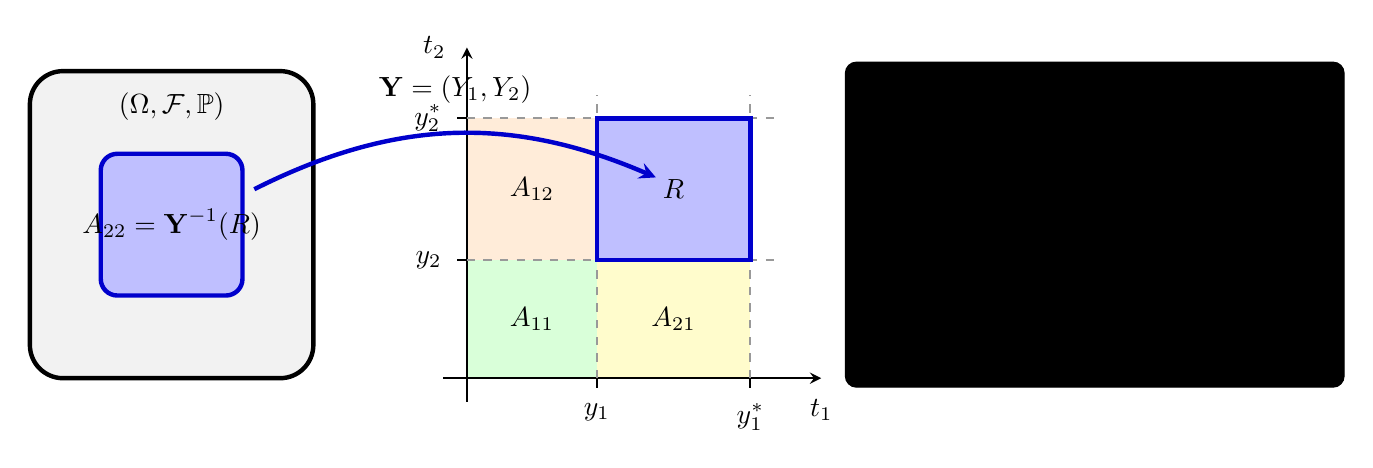
\begin{tikzpicture}[scale=1.5]
    % 1) Backgrounds / Shaded Regions
    % Sample space Omega on the left
    \fill[gray!10, rounded corners=12pt] (-3.2, 0.2) rectangle (-0.8, 2.8);
    \fill[blue!25, rounded corners=6pt] (-2.6, 0.9) rectangle (-1.4, 2.1);

    % Euclidean plane R^2 on the right: 4 disjoint blocks of F(y_1^*, y_2^*)
    \fill[green!15] (0.5, 0.2) rectangle (1.6, 1.2);
    \fill[yellow!20] (1.6, 0.2) rectangle (2.9, 1.2);
    \fill[orange!15] (0.5, 1.2) rectangle (1.6, 2.4);
    \fill[blue!25] (1.6, 1.2) rectangle (2.9, 2.4);

    % 2) Grid Lines and Axes
    \draw[->, thick, >=stealth] (0.3, 0.2) -- (3.5, 0.2) node[below=4pt, black] {$\displaystyle t_1$};
    \draw[->, thick, >=stealth] (0.5, 0.0) -- (0.5, 3.0) node[left=4pt, black] {$\displaystyle t_2$};
    \draw[dashed, thick, gray!80] (1.6, 0.2) -- (1.6, 2.6);
    \draw[dashed, thick, gray!80] (2.9, 0.2) -- (2.9, 2.6);
    \draw[dashed, thick, gray!80] (0.5, 1.2) -- (3.1, 1.2);
    \draw[dashed, thick, gray!80] (0.5, 2.4) -- (3.1, 2.4);

    % 3) Primary Plots / Borders and Pushforward Mapping Arrow
    \draw[ultra thick, black, rounded corners=12pt] (-3.2, 0.2) rectangle (-0.8, 2.8);
    \draw[ultra thick, blue!80!black, rounded corners=6pt] (-2.6, 0.9) rectangle (-1.4, 2.1);
    \draw[ultra thick, blue!80!black] (1.6, 1.2) rectangle (2.9, 2.4);
    \draw[->, ultra thick, blue!80!black, >=stealth] (-1.3, 1.8) to[bend left=25] (2.1, 1.9);

    % 4) Node Labels, Tick Marks, and Legend
    \node[black] at (-2.0, 2.5) {$\displaystyle (\Omega, \mathcal{F}, \mathbb{P})$};
    \node[black] at (-2.0, 1.5) {$\displaystyle A_{22} = \mathbf{Y}^{-1}(R)$};
    \node[above=4pt, black] at (0.4, 2.35) {$\displaystyle \mathbf{Y} = (Y_1, Y_2)$};

    \draw[thick] (1.6, 0.2) -- (1.6, 0.12) node[below=2pt, black] {$\displaystyle y_1$};
    \draw[thick] (2.9, 0.2) -- (2.9, 0.12) node[below=2pt, black] {$\displaystyle y_1^*$};
    \draw[thick] (0.5, 1.2) -- (0.42, 1.2) node[left=2pt, black] {$\displaystyle y_2$};
    \draw[thick] (0.5, 2.4) -- (0.42, 2.4) node[left=2pt, black] {$\displaystyle y_2^*$};

    \node[black] at (1.05, 0.7) {$\displaystyle A_{11}$};
    \node[black] at (2.25, 0.7) {$\displaystyle A_{21}$};
    \node[black] at (1.05, 1.8) {$\displaystyle A_{12}$};
    \node[black] at (2.25, 1.8) {$\displaystyle R$};

    \node[draw, rounded corners, fill=white, align=left, inner sep=8pt, anchor=west, black] at (3.7, 1.5) {
        \textbf{2-Increasing Decomposition}\\[4pt]
        $\displaystyle F(y_1^*, y_2^*) = \mathbb{P}(A_{11} \cup A_{12} \cup A_{21} \cup A_{22})$\\[4pt]
        $\displaystyle F(y_1^*, y_2) = \mathbb{P}(A_{11} \cup A_{21})$\\[4pt]
        $\displaystyle F(y_1, y_2^*) = \mathbb{P}(A_{11} \cup A_{12})$\\[4pt]
        $\displaystyle F(y_1, y_2) = \mathbb{P}(A_{11})$\\[4pt]
        $\displaystyle \mathbb{P}(R) = F(y_1^*, y_2^*) - F(y_1^*, y_2)$\\
        $\displaystyle \phantom{\mathbb{P}(R) =} - F(y_1, y_2^*) + F(y_1, y_2) \ge 0$
    };
\end{tikzpicture}
\end{center}

\subsection{Heuristics and ``Cheats''}

\begin{itemize}
    \item \textbf{The Uniform Density Shortcut:} Whenever $(Y_1, Y_2)$ has a constant density $f(y_1, y_2) = k$ on a support $\mathcal{S} \subseteq \mathbb{R}^2$ (as in Exercises 5.6, 5.10, 5.11, 5.12, and 5.17), you do not need calculus! Immediately use Euclidean geometry:
    \[
        k = \frac{1}{\text{Area}(\mathcal{S})}, \qquad \mathbb{P}((Y_1, Y_2) \in B) = \frac{\text{Area}(B \cap \mathcal{S})}{\text{Area}(\mathcal{S})}.
    \]
    \item \textbf{Choosing the Inner Integration Variable:} Look at two things: (1) Which variable appears in fewer boundary equations of $\mathcal{S} \cap B$? (2) Which variable makes the antiderivative easier? For example, in Exercise 5.15, $f(y_1, y_2) = e^{-y_1}$ is independent of $y_2$, so integrating with respect to $y_2$ first trivially multiplies $e^{-y_1}$ by the length of the vertical slice!
    \item \textbf{Symmetry/Exchangeability Check:} If $\mathcal{S}$ is symmetric across the line $y_1 = y_2$ and $f(y_1, y_2) = f(y_2, y_1)$ for all $(y_1, y_2) \in \mathcal{S}$ (and $(Y_1, Y_2)$ is jointly continuous), then $\mathbb{P}(Y_1 \le Y_2) = \mathbb{P}(Y_1 < Y_2) = \frac{1}{2}$ immediately without integration (as in Exercise 5.17).
\end{itemize}

\subsection{Pitfalls and Fallacies}

\begin{enumerate}[label=\textbf{\arabic*.}]
    \item \textbf{The 1D-to-2D CDF Fallacy:} Students frequently write $\mathbb{P}(a_1 < Y_1 \le b_1, a_2 < Y_2 \le b_2) = F(b_1, b_2) - F(a_1, a_2)$. \emph{This is false!} Subtracting $F(a_1, a_2)$ only removes the bottom-left quadrant $(-\infty, a_1] \times (-\infty, a_2]$, leaving two infinite strips $(-\infty, a_1] \times (a_2, b_2]$ and $(a_1, b_1] \times (-\infty, a_2]$ unaccounted for. You must use the four-term inclusion-exclusion formula: $F(b_1, b_2) - F(b_1, a_2) - F(a_1, b_2) + F(a_1, a_2)$.
    \item \textbf{Assuming Product Form Implies Independence on Non-Rectangular Supports:} In Exercise 5.5, $f(y_1, y_2) = 3y_1 = (3y_1)(1)$ looks like a factored product of a function of $y_1$ and a function of $y_2$. However, the support $0 \le y_2 \le y_1 \le 1$ couples $y_1$ and $y_2$ via the indicator $\mathbf{1}_{\{y_2 \le y_1\}}(y_1, y_2)$, which does \emph{not} factor! Thus $Y_1$ and $Y_2$ are dependent.
    \item \textbf{Confusing Mutually Exclusive Events with Independent Random Variables:} For a single realization $\omega \in \Omega$, the bivariate point events $\{Y_1 = 0, Y_2 = 0\}$ and $\{Y_1 = 1, Y_2 = 1\}$ are mutually exclusive (disjoint subsets of $\Omega$, so $\mathbb{P}(A \cap B) = 0$). Independence of $Y_1$ and $Y_2$ means $\mathbb{P}(Y_1 = y_1, Y_2 = y_2) = \mathbb{P}(Y_1 = y_1)\mathbb{P}(Y_2 = y_2)$ across all pairs.
    \item \textbf{Ignoring Piecewise Saturation in Joint CDFs:} When computing $F(y_1, y_2)$ outside the support (such as $F(1/2, 2)$ in Exercise 5.13(b)), plugging $y_2 = 2$ blindly into the antiderivative polynomial produces probabilities greater than $1$. Always cap the integration upper limit at the support boundary $\min(y_2, 1 - y_1)$.
\end{enumerate}

\newpage

\section{Conceptual Synthesis and the ``Big Picture''}

\subsection{Thematic Connections}

The unifying theme of Chapter 5.2 is \textbf{the pushforward of probability measures from abstract sample spaces to finite-dimensional Euclidean product spaces $(\mathbb{R}^n, \mathcal{B}(\mathbb{R}^n))$}. In abstract algebra and topology, we study how structure-preserving maps (homomorphisms, continuous functions) transport algebraic or topological properties from a domain to a codomain. In measure-theoretic probability, a random vector $\mathbf{Y} : (\Omega, \mathcal{F}, \mathbb{P}) \to (\mathbb{R}^n, \mathcal{B}(\mathbb{R}^n))$ is a measurable morphism that transports the abstract measure $\mathbb{P}$ into a concrete geometric measure $\mathbb{P}_{\mathbf{Y}} = \mathbb{P} \circ \mathbf{Y}^{-1}$ on $\mathbb{R}^n$.

This perspective unifies the discrete and continuous cases under a single umbrella:
\begin{itemize}
    \item In the discrete case, $\mathbb{P}_{\mathbf{Y}}$ is absolutely continuous with respect to the counting measure $\mu_c$ on a countable lattice $\mathcal{S} \subseteq \mathbb{R}^n$, and the joint PMF $p(\mathbf{y}) = \frac{d\mathbb{P}_{\mathbf{Y}}}{d\mu_c}(\mathbf{y})$ is its Radon-Nikodym derivative.
    \item In the continuous case, $\mathbb{P}_{\mathbf{Y}}$ is absolutely continuous with respect to the $n$-dimensional Lebesgue measure $\lambda_n$, and the joint PDF $f(\mathbf{y}) = \frac{d\mathbb{P}_{\mathbf{Y}}}{d\lambda_n}(\mathbf{y})$ is its Radon-Nikodym derivative.
    \item In both cases, the joint CDF $F(\mathbf{y}) = \mathbb{P}_{\mathbf{Y}}\!\left(\prod_{i=1}^n (-\infty, y_i]\right)$ uniquely characterizes the measure $\mathbb{P}_{\mathbf{Y}}$ on all of $\mathcal{B}(\mathbb{R}^n)$ by Carath\'eodory's Extension Theorem and the $\pi$-$\lambda$ Theorem (since semi-infinite boxes $\prod_{i=1}^n (-\infty, y_i]$ form a $\pi$-system generating $\mathcal{B}(\mathbb{R}^n)$).
\end{itemize}

\subsection{Forward and Backward Links}

\textbf{Backward Links (How Section 5.2 Extends Prior Concepts):}
\begin{itemize}
    \item \emph{Set Theory \& Combinatorics (Chapter 2):} Joint events $\{Y_1 = y_1, Y_2 = y_2\}$ are direct translations of set intersections $A \cap B$. Multinomial and multivariate hypergeometric PMFs (Exercises 5.1, 5.3) directly generalize binomial and univariate hypergeometric counting.
    \item \emph{Univariate Discrete \& Continuous Distributions (Chapters 3 \& 4):} Sums of point masses $\sum_y p(y) = 1$ extend to double sums $\sum_{y_1}\sum_{y_2} p(y_1, y_2) = 1$, and areas under a curve $\int_a^b f(y)\,dy$ extend to volumes under a surface $\iint_R f(y_1, y_2)\,dy_1\,dy_2$.
\end{itemize}

\textbf{Forward Links (How Section 5.2 Serves as a Bedrock for Advanced Topics):}
\begin{itemize}
    \item \emph{Marginal and Conditional Distributions (Section 5.3):} Integrating out nuisance variables ($f_{Y_1}(y_1) = \int_{-\infty}^\infty f(y_1, y_2)\,dy_2$) is the measure-theoretic projection of $\mathbb{P}_{(Y_1, Y_2)}$ onto coordinate subspaces, and conditioning ($f(y_2 \mid y_1) = \frac{f(y_1, y_2)}{f_{Y_1}(y_1)}$) is the foundation of Bayesian inference and Markov transition kernels.
    \item \emph{Expectation of Functions of Random Vectors \& Covariance (Sections 5.5--5.7):} The Law of the Unconscious Statistician (LOTUS) in $\mathbb{R}^n$, $\mathbb{E}[g(\mathbf{Y})] = \int_{\mathbb{R}^n} g(\mathbf{y}) f(\mathbf{y})\,d\mathbf{y}$, enables the definition of covariance matrices $\mathbf{\Sigma} = \mathbb{E}[(\mathbf{Y}-\boldsymbol{\mu})(\mathbf{Y}-\boldsymbol{\mu})^\top]$ and moment generating functions.
    \item \emph{Stochastic Processes \& Kolmogorov Consistency:} A continuous-time stochastic process $\{X_t\}_{t \ge 0}$ (such as Brownian motion in Quantitative Finance) is constructed by specifying a consistent family of finite-dimensional multivariate distributions $(X_{t_1}, X_{t_2}, \dots, X_{t_n})$ and invoking the Kolmogorov Extension Theorem.
\end{itemize}

\newpage

\section{Abstract Real-World Modeling (AI, ML, and Quant Finance)}

\subsection{Concrete Scenarios}

\begin{enumerate}[label=\textbf{Scenario \arabic*:}, leftmargin=1in]
    \item \textbf{Generative Artificial Intelligence (Normalizing Flows and Score-Based Diffusion Models):}
    Modern generative AI models (such as Stable Diffusion and Sora) synthesize high-resolution images by learning an intractable high-dimensional joint probability density $f_{\mathbf{Y}}(\mathbf{y})$ on $\mathbb{R}^d$ ($d \sim 10^6$). A \emph{Normalizing Flow} transforms a simple base multivariate distribution $\mathbf{Z} \sim \mathcal{N}(\mathbf{0}, \mathbf{I}_d)$ through a sequence of diffeomorphisms $\mathbf{Y} = T_\theta(\mathbf{Z})$, computing the exact joint density via the multivariate Jacobian change-of-variables formula $f_{\mathbf{Y}}(\mathbf{y}) = f_{\mathbf{Z}}(T_\theta^{-1}(\mathbf{y})) \left|\det D T_\theta^{-1}(\mathbf{y})\right|$. Score-based diffusion models perturb $\mathbf{Y}_0$ via a forward multivariate Ornstein-Uhlenbeck SDE and train a neural network to approximate the \emph{score function} $\nabla_{\mathbf{y}} \ln f_t(\mathbf{y})$.
    \item \textbf{Quantitative Finance (Multi-Asset Basket Derivatives and Copula Credit Modeling):}
    In institutional derivatives trading, exotic options such as \emph{Rainbow Options}, \emph{Spread Options} ($\max(S_T^{(1)} - S_T^{(2)} - K, 0)$), and \emph{Collateralized Debt Obligations (CDOs)} depend on the joint distribution $F(s_1, \dots, s_n)$ of multiple underlying asset prices or default times $(\tau_1, \dots, \tau_n)$ under a risk-neutral measure $\mathbb{Q}$. Notice that Exercise 5.15 (evaluating $\mathbb{P}(Y_1 - Y_2 \ge 1)$) and Exercise 5.6a ($\mathbb{P}(Y_1 - Y_2 > 0.5)$) are exact prototypes of pricing a digital spread option! By Sklar's Theorem, quants decompose any multivariate CDF into its marginals and a \emph{Copula} $C : [0,1]^n \to [0,1]$ via $F(y_1, \dots, y_n) = C(F_1(y_1), \dots, F_n(y_n))$ to capture tail dependence during market crashes.
    \item \textbf{Statistical Learning Theory and Bayesian Networks (Dirichlet-Multinomial Topic Models):}
    In Natural Language Processing and Bayesian Machine Learning, proportion vectors $\mathbf{Y} = (Y_1, \dots, Y_K)$ lying on the probability simplex $\Delta^K = \{\mathbf{y} \in [0,1]^K : \sum_{i=1}^K y_i \le 1\}$ are modeled using the \emph{Dirichlet distribution}, which directly generalizes the simplex densities in Exercises 5.5, 5.12, and 5.13!
\end{enumerate}

\subsection{Model Problem Setup: Quantitative Research Formulation of a Bivariate Spread Option and Score-Based Generative SDE}

We now formulate a rigorous mathematical model bridging Quantitative Finance (bivariate spread derivative pricing) and Stochastic Calculus.

\textbf{1. Filtered Probability Space and State Space:}
Let $(\Omega, \mathcal{F}, \{\mathcal{F}_t\}_{t \in [0, T]}, \mathbb{Q})$ be a complete filtered probability space satisfying the usual conditions, where $\mathbb{Q}$ is the unique equivalent martingale (risk-neutral) measure, and $\mathbf{W}_t = (W_t^{(1)}, W_t^{(2)})^\top$ is a two-dimensional standard $\mathbb{Q}$-Brownian motion with instantaneous correlation $\operatorname{Cov}_{\mathbb{Q}}(dW_t^{(1)}, dW_t^{(2)}) = \rho\,dt$, $\rho \in (-1, 1)$.

\textbf{2. Bivariate Stochastic Differential Equation (It\^o Diffusion):}
Let $\mathbf{S}_t = (S_t^{(1)}, S_t^{(2)})^\top \in (0, \infty)^2$ denote the prices of two correlated financial assets (e.g., Brent Crude Oil and WTI Crude Oil futures) governed by the coupled geometric Brownian motion SDE:
\[
    dS_t^{(i)} = r S_t^{(i)}\,dt + \sigma_i S_t^{(i)}\,dW_t^{(i)}, \qquad S_0^{(i)} = s_0^{(i)} > 0, \qquad i \in \{1, 2\},
\]
where $r > 0$ is the risk-free interest rate and $\sigma_1, \sigma_2 > 0$ are the asset volatilities.

\textbf{3. Derivation of the Log-Return Joint Density via It\^o's Lemma:}
Define the log-price vector $\mathbf{Y}_T = (Y_1, Y_2)^\top = (\ln(S_T^{(1)}/S_0^{(1)}), \ln(S_T^{(2)}/S_0^{(2)}))^\top$. Applying It\^o's Lemma to $\psi(s) = \ln s$,
\[
    d(\ln S_t^{(i)}) = \frac{1}{S_t^{(i)}}\,dS_t^{(i)} - \frac{1}{2(S_t^{(i)})^2}\,d\langle S^{(i)}, S^{(i)}\rangle_t = \left(r - \frac{1}{2}\sigma_i^2\right)dt + \sigma_i\,dW_t^{(i)}.
\]
Integrating from $t = 0$ to $t = T$ shows that $\mathbf{Y}_T$ follows a bivariate Gaussian distribution $\mathcal{N}_2(\boldsymbol{\mu}, \mathbf{\Sigma})$ on $(\mathbb{R}^2, \mathcal{B}(\mathbb{R}^2))$ with mean vector $\boldsymbol{\mu}$ and covariance matrix $\mathbf{\Sigma}$:
\[
    \boldsymbol{\mu} = \begin{bmatrix} \mu_1 \\ \mu_2 \end{bmatrix} = \begin{bmatrix} \left(r - \frac{1}{2}\sigma_1^2\right)T \\[4pt] \left(r - \frac{1}{2}\sigma_2^2\right)T \end{bmatrix}, \qquad
    \mathbf{\Sigma} = \begin{bmatrix} \sigma_1^2 T & \rho \sigma_1 \sigma_2 T \\[4pt] \rho \sigma_1 \sigma_2 T & \sigma_2^2 T \end{bmatrix}.
\]
The joint probability density function $f_{(Y_1, Y_2)}(y_1, y_2) = \frac{d\mathbb{Q}_{(Y_1, Y_2)}}{d\lambda_2}$ is explicitly given by:
\[
    f(y_1, y_2) = \frac{1}{2\pi \sigma_1 \sigma_2 T \sqrt{1 - \rho^2}} \exp\!\left( -\frac{1}{2(1 - \rho^2)T} \left[ \frac{(y_1 - \mu_1)^2}{\sigma_1^2} - \frac{2\rho(y_1 - \mu_1)(y_2 - \mu_2)}{\sigma_1 \sigma_2} + \frac{(y_2 - \mu_2)^2}{\sigma_2^2} \right] \right).
\]

\textbf{4. Arbitrage-Free Pricing Integral and Score-Matching Loss Function:}
Consider a European Spread Call Option with strike $K \ge 0$ and maturity $T$, whose terminal payoff is $\Phi(S_T^{(1)}, S_T^{(2)}) = \max\!\left(S_T^{(1)} - S_T^{(2)} - K, 0\right)$. By the First Fundamental Theorem of Asset Pricing, its arbitrage-free price at $t = 0$ is the discounted bivariate integral over the non-rectangular exercise domain $R_K = \{(y_1, y_2) \in \mathbb{R}^2 : s_0^{(1)} e^{y_1} - s_0^{(2)} e^{y_2} > K\}$:
\[
    V_0 = e^{-rT} \mathbb{E}_{\mathbb{Q}}\!\left[\Phi(S_T^{(1)}, S_T^{(2)})\right] = e^{-rT} \int_{-\infty}^{\infty} \int_{\ln\!\left(\frac{s_0^{(2)} e^{y_2} + K}{s_0^{(1)}}\right)}^{\infty} \left( s_0^{(1)} e^{y_1} - s_0^{(2)} e^{y_2} - K \right) f(y_1, y_2)\, dy_1\, dy_2.
\]
When the parametric form of $f(y_1, y_2)$ is unknown and must be learned from market order-flow data using a Score-Based Generative Neural Network $\mathbf{s}_\theta : \mathbb{R}^2 \to \mathbb{R}^2$, we minimize the \emph{Hyv\"arinen Score-Matching Optimization Objective} (which bypasses computing the intractable normalizing constant $k$ of Section 5.2 via multivariate integration by parts / divergence theorem):
\[
    \min_{\theta \in \Theta} \mathcal{L}(\theta) = \mathbb{E}_{(Y_1, Y_2) \sim f}\!\left[ \frac{1}{2} \bigl\| \mathbf{s}_\theta(Y_1, Y_2) \bigr\|_2^2 + \operatorname{tr}\!\bigl( \nabla_{\mathbf{y}} \mathbf{s}_\theta(Y_1, Y_2) \bigr) \right].
\]

\newpage

\section{Common Variations and Untested Concepts}

A standard advanced university curriculum on Multivariate Probability Distributions includes three critical theoretical concepts not tested in Exercises 5.1--5.18:
\begin{enumerate}[label=\textbf{\arabic*.}]
    \item \textbf{Recovering the Joint PDF from the Joint CDF via Mixed Partial Derivatives} ($\frac{\partial^2 F}{\partial y_1 \partial y_2}$).
    \item \textbf{Singular and Mixed Bivariate Distributions} (Failures of Radon-Nikodym absolute continuity where $\mathbb{P}(Y_1 = Y_2) > 0$).
    \item \textbf{Multivariate Jacobian Change-of-Variables Theorem} for nonlinear transformations of random vectors.
\end{enumerate}
Below, we provide a rigorous theorem and complete worked proof/example for each concept.

\subsection{Untested Concept 1: Recovering $f(y_1, y_2)$ and Rectangle Probabilities from a Non-Separable Joint CDF}

\begin{example}[Mixed Partial Differentiation and 2-Increasing Evaluation]
Let $(Y_1, Y_2)$ be non-negative random variables with joint cumulative distribution function (the bivariate Gumbel-Barnett survival/CDF family):
\[
    F(y_1, y_2) = \begin{cases}
        1 - e^{-y_1} - e^{-y_2} + e^{-(y_1 + y_2 + \theta y_1 y_2)}, & y_1 \ge 0,\ y_2 \ge 0, \\
        0, & \text{elsewhere,}
    \end{cases}
\]
where $\theta \in [0, 1]$ is a dependence parameter.
\begin{enumerate}[label=(\alph*)]
    \item Derive the joint probability density function $f(y_1, y_2)$ and prove that $f(y_1, y_2) \ge 0$ for all $y_1, y_2 \ge 0$ when $\theta \in [0, 1]$.
    \item Compute $\mathbb{P}(1 < Y_1 \le 2, 1 < Y_2 \le 2)$ directly from $F(y_1, y_2)$ for $\theta = \frac{1}{2}$.
\end{enumerate}
\end{example}

\begin{proof}[Solution and Proof]
\textbf{Part (a):} By the Fundamental Theorem of Calculus and Clairaut's Theorem on mixed partial derivatives, for $y_1 > 0$ and $y_2 > 0$,
\[
    \frac{\partial F(y_1, y_2)}{\partial y_1} = e^{-y_1} - (1 + \theta y_2) e^{-(y_1 + y_2 + \theta y_1 y_2)}.
\]
Differentiating with respect to $y_2$ yields the joint PDF:
\begin{align*}
    f(y_1, y_2) &= \frac{\partial^2 F(y_1, y_2)}{\partial y_2 \partial y_1} \\
    &= -\theta e^{-(y_1 + y_2 + \theta y_1 y_2)} + (1 + \theta y_2)(1 + \theta y_1) e^{-(y_1 + y_2 + \theta y_1 y_2)} \\
    &= \bigl[ (1 + \theta y_1)(1 + \theta y_2) - \theta \bigr] e^{-(y_1 + y_2 + \theta y_1 y_2)} \\
    &= \bigl( 1 - \theta + \theta y_1 + \theta y_2 + \theta^2 y_1 y_2 \bigr) e^{-(y_1 + y_2 + \theta y_1 y_2)}.
\end{align*}
Since $\theta \in [0, 1]$, we have $1 - \theta \ge 0$, and since $y_1, y_2 \ge 0$, every term inside the parenthesis is non-negative. Thus $f(y_1, y_2) \ge 0$ on $\mathbb{R}^2$.

\textbf{Part (b):} By Theorem 5.2a (Part 3), for $\theta = \frac{1}{2}$,
\begin{align*}
    \mathbb{P}(1 < Y_1 \le 2, 1 < Y_2 \le 2) &= F(2, 2) - F(2, 1) - F(1, 2) + F(1, 1) \\
    &= e^{-(2 + 2 + 2)} - 2 e^{-(2 + 1 + 1)} + e^{-(1 + 1 + 1/2)} \\
    &= e^{-6} - 2e^{-4} + e^{-5/2}.
\end{align*}
\end{proof}

\subsection{Untested Concept 2: Singular Bivariate Distributions and Lebesgue Decomposition}

\begin{proposition}[Continuous Marginals Without Joint Absolute Continuity]
Let $U \sim \text{Uniform}(0, 1)$, and define the bivariate random vector $(Y_1, Y_2) = (U, U)$. Prove that $Y_1$ and $Y_2$ are each continuous random variables, yet $(Y_1, Y_2)$ is \emph{not} jointly continuous (it possesses no joint PDF $f(y_1, y_2)$ with respect to two-dimensional Lebesgue measure $\lambda_2$), and find its joint CDF $F(y_1, y_2)$.
\end{proposition}

\begin{proof}
For each $i \in \{1, 2\}$, $F_{Y_i}(y) = \mathbb{P}(U \le y) = y$ for $y \in [0, 1]$, which is continuous everywhere with univariate PDF $f_{Y_i}(y) = \mathbf{1}_{[0, 1]}(y)$. However, the joint CDF of $(Y_1, Y_2)$ for $y_1, y_2 \in [0, 1]$ is:
\[
    F(y_1, y_2) = \mathbb{P}(U \le y_1, U \le y_2) = \mathbb{P}(U \le \min(y_1, y_2)) = \min(y_1, y_2).
\]
Suppose toward a contradiction that $(Y_1, Y_2)$ admits a joint density $f(y_1, y_2)$ satisfying Definition 5.3. Consider the diagonal line segment $D = \{(t, t) : t \in [0, 1]\} \subseteq \mathbb{R}^2$. Because $D$ is a one-dimensional line segment in $\mathbb{R}^2$, its two-dimensional Lebesgue measure is $\lambda_2(D) = \int_0^1 \int_t^t 1\,dy_2\,dy_1 = 0$. Any integral of a Lebesgue-integrable function $f$ over a set of $\lambda_2$-measure zero must be zero:
\[
    \iint_{D} f(y_1, y_2)\,dy_1\,dy_2 = 0.
\]
Yet by construction, $Y_1(\omega) = U(\omega) = Y_2(\omega)$ for all $\omega \in \Omega$, so $\mathbb{P}((Y_1, Y_2) \in D) = \mathbb{P}(U = U) = 1 \neq 0$, a contradiction! In measure theory, $\mathbb{P}_{(Y_1, Y_2)}$ is \emph{mutually singular} with respect to $\lambda_2$ ($\mathbb{P}_{(Y_1, Y_2)} \perp \lambda_2$), concentrating all its mass on the 1D manifold $D$.
\end{proof}

\subsection{Untested Concept 3: Bivariate Jacobian Change-of-Variables Theorem}

\begin{theorem}[Bivariate Change of Variables]
Let $(Y_1, Y_2)$ be jointly continuous with joint PDF $f_{Y_1, Y_2}(y_1, y_2)$ supported on an open set $\mathcal{S} \subseteq \mathbb{R}^2$. Let $\mathbf{g} = (g_1, g_2) : \mathcal{S} \to \mathcal{T}$ be a $C^1$-diffeomorphism onto $\mathcal{T} = \mathbf{g}(\mathcal{S})$ with inverse $\mathbf{h}(u_1, u_2) = (h_1(u_1, u_2), h_2(u_1, u_2))$. Then the transformed random vector $(U_1, U_2) = \mathbf{g}(Y_1, Y_2)$ is jointly continuous with joint PDF:
\[
    f_{U_1, U_2}(u_1, u_2) = f_{Y_1, Y_2}\bigl(h_1(u_1, u_2), h_2(u_1, u_2)\bigr) \cdot \bigl| J(u_1, u_2) \bigr| \, \mathbf{1}_{\mathcal{T}}(u_1, u_2),
\]
where $J(u_1, u_2) = \det \begin{bmatrix} \frac{\partial h_1}{\partial u_1} & \frac{\partial h_1}{\partial u_2} \\[4pt] \frac{\partial h_2}{\partial u_2} & \frac{\partial h_2}{\partial u_2} \end{bmatrix} = \frac{\partial h_1}{\partial u_1}\frac{\partial h_2}{\partial u_2} - \frac{\partial h_1}{\partial u_2}\frac{\partial h_2}{\partial u_1}$ is the Jacobian determinant of the inverse map.
\end{theorem}

\begin{example}[Worked Application to Exercise 5.7]
In Exercise 5.7, $f_{Y_1, Y_2}(y_1, y_2) = e^{-(y_1 + y_2)}$ for $y_1 > 0, y_2 > 0$. Define $U_1 = Y_1 + Y_2$ (the total lifetime) and $U_2 = \frac{Y_1}{Y_1 + Y_2}$ (the proportion of lifetime from component 1). Find the joint PDF of $(U_1, U_2)$.
\end{example}

\begin{proof}[Solution]
The inverse transformation mapping $\mathcal{T} = (0, \infty) \times (0, 1)$ onto $\mathcal{S} = (0, \infty)^2$ is $y_1 = h_1(u_1, u_2) = u_1 u_2$ and $y_2 = h_2(u_1, u_2) = u_1(1 - u_2)$. The Jacobian determinant is:
\[
    J(u_1, u_2) = \det \begin{bmatrix} u_2 & u_1 \\ 1 - u_2 & -u_1 \end{bmatrix} = -u_1 u_2 - u_1(1 - u_2) = -u_1 \implies |J(u_1, u_2)| = u_1.
\]
By Theorem 7.1, the joint PDF of $(U_1, U_2)$ is:
\[
    f_{U_1, U_2}(u_1, u_2) = e^{-(u_1 u_2 + u_1(1 - u_2))} \cdot u_1 = u_1 e^{-u_1} \, \mathbf{1}_{(0, \infty)}(u_1) \, \mathbf{1}_{(0, 1)}(u_2).
\]
Notice that integrating $f_{U_1, U_2}$ over $u_1 \in (0, 3)$ and $u_2 \in (0, 1)$ immediately gives $\mathbb{P}(Y_1 + Y_2 < 3) = \int_0^3 u_1 e^{-u_1}\,du_1 = 1 - 4e^{-3}$, matching our solution to Exercise 5.7(b)!
\end{proof}

\newpage

\section{Advanced Diagnostic Testing: ``Find the Flaw''}

Below are five advanced problems accompanied by seemingly rigorous step-by-step proofs/solutions. However, \textbf{each proof contains a single, subtle, yet fatal mathematical or logical flaw}. Act as the grader: identify the exact line where the error occurs, explain why it violates probability or measure theory, and provide the corrected calculation.

\subsection{Diagnostic Problems and Flawed Proofs}

\subsubsection*{Diagnostic Problem 1: Validity of a Proposed Bivariate CDF}
\textbf{Problem:} Let $F : \mathbb{R}^2 \to [0, 1]$ be defined by
\[
    F(y_1, y_2) = \begin{cases}
        0, & \text{if } y_1 < 0,\ y_2 < 0,\ \text{or } y_1 + y_2 < 1, \\
        1, & \text{if } y_1 \ge 0,\ y_2 \ge 0,\ \text{and } y_1 + y_2 \ge 1.
    \end{cases}
\]
Determine whether $F(y_1, y_2)$ is a valid joint cumulative distribution function.

\textbf{Proposed Proof:}
\begin{enumerate}[label=\textbf{Step \arabic*:}]
    \item Check boundary limits at $-\infty$: If $y_1 \to -\infty$ or $y_2 \to -\infty$, then $y_1 < 0$ or $y_2 < 0$, so $F(-\infty, y_2) = F(y_1, -\infty) = F(-\infty, -\infty) = 0$.
    \item Check limit at $+\infty$: As $y_1 \to \infty$ and $y_2 \to \infty$, we have $y_1 \ge 0, y_2 \ge 0$, and $y_1 + y_2 \ge 1$, so $F(\infty, \infty) = 1$.
    \item Check coordinate-wise monotonicity: Fix $y_2 \in \mathbb{R}$. If $y_1 < y_1^*$, then $y_1 + y_2 < y_1^* + y_2$, so $F(y_1, y_2) \le F(y_1^*, y_2)$ because the indicator of $\{y_1 + y_2 \ge 1\}$ is non-decreasing in $y_1$. By symmetry, $F(y_1, y_2)$ is also non-decreasing in $y_2$.
    \item Check right-continuity: Since the region $\{y_1 \ge 0, y_2 \ge 0, y_1 + y_2 \ge 1\}$ is closed with weak inequalities $\ge$, approaching any point $(y_1, y_2)$ from above ($h_1, h_2 \to 0^+$) preserves the inequalities, so $F$ is right-continuous in both arguments.
    \item \textbf{Conclusion:} Since $F$ satisfies $0 \le F \le 1$, boundary limits, right-continuity, and coordinate-wise monotonicity in $y_1$ and $y_2$, $F(y_1, y_2)$ is a valid joint CDF. $\blacksquare$
\end{enumerate}

\bigskip

\subsubsection*{Diagnostic Problem 2: Computing a Rectangular Probability from a Joint CDF}
\textbf{Problem:} Let $(Y_1, Y_2)$ have the valid joint CDF from Exercise 5.8, where $F(y_1, y_2) = y_1^2 y_2^2$ on $[0, 1]^2$. Compute $\mathbb{P}(1/2 < Y_1 \le 1, 1/2 < Y_2 \le 1)$.

\textbf{Proposed Solution:}
\begin{enumerate}[label=\textbf{Step \arabic*:}]
    \item Define the cumulative events $B = \{Y_1 \le 1, Y_2 \le 1\}$ and $A = \{Y_1 \le 1/2, Y_2 \le 1/2\}$.
    \item Since $1/2 \le 1$, we have the set inclusion $A \subseteq B$, with $\mathbb{P}(B) = F(1, 1) = 1$ and $\mathbb{P}(A) = F(1/2, 1/2) = (1/2)^2(1/2)^2 = \frac{1}{16}$.
    \item By the subtractive property of probability measures for nested sets ($A \subseteq B \implies \mathbb{P}(B \setminus A) = \mathbb{P}(B) - \mathbb{P}(A)$), the probability that $Y_1$ and $Y_2$ exceed $1/2$ inside $[0, 1]^2$ is:
    \[
        \mathbb{P}(1/2 < Y_1 \le 1, 1/2 < Y_2 \le 1) = F(1, 1) - F(1/2, 1/2) = 1 - \frac{1}{16} = \frac{15}{16}. \quad \blacksquare
    \]
\end{enumerate}

\bigskip

\subsubsection*{Diagnostic Problem 3: Evaluating a Probability on a Coupled Support}
\textbf{Problem:} Let $(Y_1, Y_2)$ have the joint density function from Exercise 5.5:
\[
    f(y_1, y_2) = \begin{cases}
        3y_1, & 0 \le y_2 \le y_1 \le 1, \\
        0, & \text{elsewhere.}
    \end{cases}
\]
Compute $\mathbb{P}(Y_1 \le 3/4, Y_2 \ge 1/4)$.

\textbf{Proposed Solution:}
\begin{enumerate}[label=\textbf{Step \arabic*:}]
    \item The event $E$ specifies the bounds $0 \le Y_1 \le 3/4$ and $1/4 \le Y_2 \le 1$ (since $0 \le y_2 \le 1$ on the support).
    \item By Theorem 5.2b, we integrate the density formula $3y_1$ over the specified intervals for $y_1$ and $y_2$:
    \[
        \mathbb{P}(Y_1 \le 3/4, Y_2 \ge 1/4) = \int_{0}^{3/4} \int_{1/4}^{1} 3y_1 \, dy_2 \, dy_1.
    \]
    \item Evaluating the inner and outer integrals:
    \[
        \int_{0}^{3/4} 3y_1 \left(1 - \frac{1}{4}\right) dy_1 = \frac{9}{4} \left[ \frac{1}{2} y_1^2 \right]_{0}^{3/4} = \frac{9}{8} \left(\frac{9}{16}\right) = \frac{81}{128}. \quad \blacksquare
    \]
\end{enumerate}

\bigskip

\subsubsection*{Diagnostic Problem 4: Fubini's Theorem on an Unbounded Bivariate Function}
\textbf{Problem:} Suppose a researcher proposes the bivariate function on $(0, 1]^2$:
\[
    h(y_1, y_2) = \frac{y_1^2 - y_2^2}{(y_1^2 + y_2^2)^2}, \qquad 0 < y_1 \le 1,\ 0 < y_2 \le 1,
\]
as a zero-mean perturbation to a uniform density $f(y_1, y_2) = 1 + c h(y_1, y_2)$, claiming that $\int_0^1 \int_0^1 h(y_1, y_2)\,dy_2\,dy_1 = 0$ by Fubini's Theorem. Verify their integration.

\textbf{Proposed Proof:}
\begin{enumerate}[label=\textbf{Step \arabic*:}]
    \item Observe the partial derivative identity: $\frac{\partial}{\partial y_2}\!\left( \frac{y_2}{y_1^2 + y_2^2} \right) = \frac{(y_1^2 + y_2^2) - y_2(2y_2)}{(y_1^2 + y_2^2)^2} = \frac{y_1^2 - y_2^2}{(y_1^2 + y_2^2)^2}$.
    \item Integrate with respect to $y_2$ first for each $y_1 \in (0, 1]$, and then integrate with respect to $y_1$:
    \[
        \int_{0}^{1} \left( \int_{0}^{1} \frac{y_1^2 - y_2^2}{(y_1^2 + y_2^2)^2} \, dy_2 \right) dy_1 = \int_{0}^{1} \left[ \frac{y_2}{y_1^2 + y_2^2} \right]_{y_2=0}^{y_2=1} dy_1 = \int_{0}^{1} \frac{1}{y_1^2 + 1} \, dy_1 = \arctan(1) = \frac{\pi}{4}.
    \]
    \item By Fubini's Theorem, the double integral over $[0, 1]^2$ is well-defined and equals $\frac{\pi}{4}$. $\blacksquare$
\end{enumerate}

\bigskip

\subsubsection*{Diagnostic Problem 5: Piecewise Joint CDF Construction}
\textbf{Problem:} For the joint PDF $f(y_1, y_2) = 2$ on the simplex $\mathcal{S} = \{y_1 \ge 0, y_2 \ge 0, y_1 + y_2 \le 1\}$ (Exercise 5.12), find the formula for the joint CDF $F(y_1, y_2)$ valid for all $(y_1, y_2) \in [0, 1]^2$.

\textbf{Proposed Solution:}
\begin{enumerate}[label=\textbf{Step \arabic*:}]
    \item Let $(y_1, y_2) \in [0, 1]^2$. By Definition 5.3, we integrate $f(t_1, t_2) = 2$ over $0 \le t_1 \le y_1$ and $0 \le t_2 \le y_2$:
    \[
        F(y_1, y_2) = \int_{0}^{y_1} \int_{0}^{y_2} 2 \, dt_2 \, dt_1 = 2 y_1 y_2 \qquad \forall (y_1, y_2) \in [0, 1]^2. \quad \blacksquare
    \]
\end{enumerate}

\newpage

\subsection{Solution Key and Grader's Critique}

\begin{enumerate}[label=\textbf{Critique of Diagnostic Problem \arabic*:}, leftmargin=0pt, itemindent=0pt]
    \item \textbf{Flaw Located in Step 3 / Step 5 (Confusing Coordinate-Wise Monotonicity with Planar 2-Increasing Monotonicity).}
    \begin{itemize}
        \item \emph{Why it is an error:} In $\mathbb{R}^2$, coordinate-wise monotonicity ($F$ non-decreasing in $y_1$ and $y_2$ separately) is \textbf{not sufficient} to guarantee that $F$ is a valid joint CDF! A valid joint CDF must satisfy Theorem 5.2a, Part 3 (the 2-increasing property): $\Delta F = F(y_1^*, y_2^*) - F(y_1^*, y_2) - F(y_1, y_2^*) + F(y_1, y_2) \ge 0$ for all $y_1^* \ge y_1$ and $y_2^* \ge y_2$.
        \item \emph{True Resolution:} Choose $y_1 = \frac{1}{3}, y_1^* = \frac{2}{3}$ and $y_2 = \frac{1}{3}, y_2^* = \frac{2}{3}$. Then:
        \[
            F\!\left(\frac{2}{3}, \frac{2}{3}\right) - F\!\left(\frac{2}{3}, \frac{1}{3}\right) - F\!\left(\frac{1}{3}, \frac{2}{3}\right) + F\!\left(\frac{1}{3}, \frac{1}{3}\right) = 1 - 1 - 1 + 0 = -1 < 0!
        \]
        This assigns a negative probability of $-1$ to the rectangle $(1/3, 2/3] \times (1/3, 2/3]$, proving $F(y_1, y_2)$ is \textbf{not} a valid joint CDF.
    \end{itemize}

    \item \textbf{Flaw Located in Step 3 (Set-Difference Fallacy on Product Spaces).}
    \begin{itemize}
        \item \emph{Why it is an error:} The set difference $B \setminus A = \{Y_1 \le 1, Y_2 \le 1\} \setminus \{Y_1 \le 1/2, Y_2 \le 1/2\}$ is the L-shaped region $\{ (Y_1 > 1/2 \lor Y_2 > 1/2) \land Y_1 \le 1 \land Y_2 \le 1\}$, \textbf{not} the logical conjunction $\{1/2 < Y_1 \le 1 \land 1/2 < Y_2 \le 1\}$! De Morgan's Law states $(E_1 \cap E_2)^c = E_1^c \cup E_2^c \neq E_1^c \cap E_2^c$.
        \item \emph{True Resolution:} Using Theorem 5.2a (Part 3),
        \[
            \mathbb{P}\!\left(\frac{1}{2} < Y_1 \le 1, \frac{1}{2} < Y_2 \le 1\right) = F(1, 1) - F\!\left(1, \frac{1}{2}\right) - F\!\left(\frac{1}{2}, 1\right) + F\!\left(\frac{1}{2}, \frac{1}{2}\right) = 1 - \frac{1}{4} - \frac{1}{4} + \frac{1}{16} = \frac{9}{16}.
        \]
    \end{itemize}

    \item \textbf{Flaw Located in Step 1 / Step 2 (Omitting the Support Indicator $\mathbf{1}_{\{y_2 \le y_1\}}$).}
    \begin{itemize}
        \item \emph{Why it is an error:} The density $f(y_1, y_2)$ equals $3y_1$ \textbf{only} when $y_2 \le y_1$, and equals $0$ when $y_2 > y_1$. By integrating over $[0, 3/4] \times [1/4, 1]$, the flawed proof integrates $3y_1$ over regions where $y_2 > y_1$ (where $f = 0$).
        \item \emph{True Resolution:} Intersecting $\{y_1 \le 3/4, y_2 \ge 1/4\}$ with $\{0 \le y_2 \le y_1 \le 1\}$ gives $1/4 \le y_2 \le y_1 \le 3/4$:
        \[
            \mathbb{P}\!\left(Y_1 \le \frac{3}{4}, Y_2 \ge \frac{1}{4}\right) = \int_{1/4}^{3/4} \int_{1/4}^{y_1} 3y_1 \, dy_2 \, dy_1 = \int_{1/4}^{3/4} 3y_1\left(y_1 - \frac{1}{4}\right) dy_1 = \left[ y_1^3 - \frac{3}{8} y_1^2 \right]_{1/4}^{3/4} = \frac{25}{128}.
        \]
    \end{itemize}

    \item \textbf{Flaw Located in Step 3 (Violation of Absolute Integrability Hypothesis in Fubini's Theorem).}
    \begin{itemize}
        \item \emph{Why it is an error:} Fubini's Theorem requires $\iint_{[0,1]^2} |h(y_1, y_2)|\,dy_1\,dy_2 < \infty$ (or $h \ge 0$ for Tonelli's Theorem). Here, $h$ takes both positive and negative values and has a non-integrable singularity at $(0, 0)$. Reversing the order of integration yields $-\frac{\pi}{4} \neq \frac{\pi}{4}$!
        \item \emph{True Resolution:} By converting to polar coordinates or integrating $|h|$, $\int_0^1 \int_0^1 |h(y_1, y_2)|\,dy_2\,dy_1 = \int_0^1 \frac{1}{y_1 (1+y_1^2)}\,dy_1 = +\infty$. Thus $h \notin L^1([0,1]^2)$, Fubini's Theorem does not apply, and $1 + c h(y_1, y_2)$ cannot be a valid PDF on $(0,1]^2$ for any $c \neq 0$ (since $h \to -\infty$ along $y_1 = 0$).
    \end{itemize}

    \item \textbf{Flaw Located in Step 1 (Failure to Bifurcate $[0,1]^2$ Along the Diagonal $y_1 + y_2 = 1$).}
    \begin{itemize}
        \item \emph{Why it is an error:} As proven in Exercise 5.12(a) and 5.12(b), the rectangle $[0, y_1] \times [0, y_2]$ is contained inside the support $\mathcal{S} = \{t_1 + t_2 \le 1\}$ \textbf{if and only if} $y_1 + y_2 \le 1$. When $y_1 + y_2 > 1$ (e.g., $y_1 = y_2 = 3/4$), the formula $2y_1 y_2$ gives $2(9/16) = 9/8 > 1$, violating $F \le 1$!
        \item \emph{True Resolution:} For $(y_1, y_2) \in [0, 1]^2$, we must split into two cases:
        \[
            F(y_1, y_2) = \begin{cases}
                2 y_1 y_2, & \text{if } 0 \le y_1 + y_2 \le 1, \\
                1 - (1 - y_1)^2 - (1 - y_2)^2 = 2y_1 + 2y_2 - y_1^2 - y_2^2 - 1, & \text{if } 1 < y_1 + y_2 \le 2.
            \end{cases}
        \]
        Checking $(y_1, y_2) = (3/4, 3/4)$ in the second branch yields $1 - (1/4)^2 - (1/4)^2 = \frac{7}{8}$, matching Exercise 5.12(a)!
    \end{itemize}
\end{enumerate}

\end{document}